\section{Introduction}
We receive a continuous stream of sensory information in our daily lives. In order to make sense of it, we often parse it into meaningful chunks for storage, retrieval and comprehension. For example, we may recall our drive to work as a series of discrete events; got into the car, got coffee, picked up a collegue, hit traffic on a particular street, parked, and walked over to the office. What aspects of the incoming stream help us organize continuous temporal information in such discrete chunks? 
Temporal chunking in cognitive psychology has been studied under several domains from event boundaries \cite{clewett2019transcending, zacks2007event, rouhani2020reward,rouhani2018dissociable,dubrow2013influence,baldwin2008segmenting}, language learning, \cite{romberg2010statistical,knowlton1992intact}, categorization \cite{unger2022ready,gabay2015incidental}, and motor sequencing \cite{bera2021motor, tremblay2010movement, savalia2016unified,ostlund2009evidence}. Chunking a repeated sequence of experiences is crucial to abstracting patterns in the environment and formation of habits for quick and efficient interactions with the environment \cite{dezfouli2012habits, smith2016habit,dolan2013goals, dezfouli2014habits, gershman2010learning, botvinick2012hierarchical}. 

Models of temporal event segmentation suggest that the points which lead to temporal segmentation seem to be unique in their properties in both segmenting the continuous stream of information and integration of information across the temporal event. These `event boundaries' are, for example, shown to be remembered better \cite{swallow2009event,rouhani2018dissociable,rouhani2018dissociable, zacks2020event, radvansky2017event, heusser2018perceptual}, serve as points of retrieval \cite{michelmann2023evidence} and replay to promote long term memory \cite{hahamy2023human, sols2017event} and easy parsing, help integrate memory across time \cite{clewett2019transcending}, and separates across boundary events while collapsing within boundary events \cite{clewett2019transcending, lositsky2016neural,ezzyat2014similarity, brunec2018boundaries}. 

In most prior studies, event boundaries have been studied using explicit context shifts. For example, when stream of stimuli are surrounded by colored border, event boundaries are operationalized by first showing the stimuli surrounded by a color and abruptly changing that color\cite{heusser2018perceptual}. In another study, event boundaries were operationalized via explicit context changes by changing the associated stimulus\cite{ezzyat2014similarity}. A pair of images were presented on each trial; one image of the pair, the 'scene' image remained constant for a short sequence of trials whereas the other ('object' or 'face') changed on each trial. Participants were asked to make judgments about the object/face image \cite{ezzyat2014similarity}. Previously, context changes had been operationalized as either perceptual or semantic shift in ongoing set of events by having participants watch clips \cite{swallow2009event}. In more recent work, context change has been operationalized as changes in ongoing reward contingencies associated with each stimulus \cite{rouhani2020reward}. 

Consistent findings across most studies in explicitly operationalized event boundaries show that event boundaries are often remembered better \cite{swallow2009event, radvansky2017event, heusser2018perceptual,clewett2019transcending, rouhani2020reward,ezzyat2014similarity,baldassano2017discovering}, and events across boundaries appear to be perceptually farther whereas events within boundaries appear to be perceptually closer \cite{clewett2019transcending,ezzyat2014similarity,brunec2018boundaries,lositsky2016neural}. In recent work, however, it has been shown that event boundaries can also be formed \textit{without} explicit changes in context. After being exposed to a stream of stimuli such that the ordering is controlled by a modular graph shown in figure \ref{fig:modular_graph}, participants seem to recognize across cluster transitions as `natural breaks' more often than within cluster transitions \cite{schapiro2013neural}. In recent work, this finding has been linked to statistical learning of temporal graph structures \cite{karuza2022value,karuza2019human,kahn2018network,kahn2018network,lynn2020abstract,lynn2020human,lynn2020humans} and measured by slowed reaction times across clusters than within clusters. However, past studies where boundaries are operationalized implicitly do not assess the memory representations of these boundaries using the same tests used in explicitly operationalized boundary paradigms. 

In this chapter, I present two tests on implicitly operationalized boundaries to assess whether they elicit the same behavioral properties as the explicitly operationalized boundaries. In particular, I use the paradigm and graph structure previously used in Schapiro et al. \cite{schapiro2013neural} to test whether participants recall boundary items better (or worse) than non-boundary items. I then use a two module graph structure in Figure \ref{fig:two_module_graph} to test whether items across the two clusters appear farther than items within a cluster (similar to findings in explicitly operationalized boundary paradigms). 

\section{Modeling Boundary Memory Benefits}
Event segmentation theory suggests that the segmentation of the continuous sensory experience occurs automatically and through prediction errors\cite{zacks2007event,zacks2007eventp, swallow2009event}. According to the event segmentation theory, we maintain an ongoing `context' which is predictive of upcoming events. Event boundaries are created when this prediction breaks. More recent work has shown that prediction errors are not necessary for creation of event boundaries; a change in uncertainty of the upcoming events can also produce event boundaries \cite{shin2021structuring}. Prediction errors particularly lose their value in learning new information when the explored environment is uncertain\cite{behrens2007learning}. Nevertheless, under environments with high regularities, prediction errors remain the key mechanisms driving boundary formation. 

As reviewed above, prediction errors need not be explicitly operationalized for an event boundary to be learned. Prediction errors which imply shifts in ongoing context, similar to implicitly operationalized event boundaries may be implicit. In chapter \ref{chapter-2-walk-lengths-modulate-statistical-learning} show that context models can be used to estimate representations of implicitly operationalized event boundaries. Particularly, predictive representations such as the SR provide a natural representation of event boundaries which form bottlenecks in transitioning between clusters in modular graphs in figure \ref{fig:modular_graph}. I propose that the same predictive context-representation framework using the Successor Representation model of Reinforcement Learning \cite{dayan1993improving, momennejad2017successor, russek2017predictive, momennejad2020learning,gershman2012successor} can be used to model differences in memory representations. 

To simulate a recognition memory task, I employ a simplified version of the exemplar-based Generalized Context Model \cite{nosofsky2011generalized,nosofsky1986attention, nosofsky2011short}. The GCM follows a class of global matching exemplar models where each studied item is stored as an image or an exemplar in memory. At test, the presented test item is matched with memory representations of stored exemplars by computing the psychological similarity between them. It is assumed that if the similarity, summed over all similarities of the test items with exemplars in memory, crosses a criterion (a free parameter), the participant recognizes that item and the `old' response is chosen in the old/new recognition test. Similarly, a `new' response is chosen when the summed similarity of the test item with all stored exemplars falls below the decision criterion. 

The GCM model for recognition memory can be formalized with the following equations \cite{nosofsky2011short}:

\begin{equation}
    \begin{aligned}
        d_{ij} = [\sum\limits_{k = 1}^K w_k(x_{ik} - x_{jk})^2]^{1/2} \\
        s_{ij} = \exp^{-c_jd_{ij}} \\
        a_{ij} = m_js_{ij}
    \end{aligned}
\end{equation}    

where $d_{ij}$ is the psychological distance between test item $i$ and examplar $j$, $w_k$ is the weight a participant may place on the $k^{th}$ dimensions (and $k \in K$). The distance metric is thus computed as an euclidean distance between exemplars in memory and the test item weighted by where each feature is allowed to have a different weight to reflect differentially important features. $s{ij}$ is the similarity between test item $i$ and exemplar $j$ which decreases exponentially with psychological distance. $c_j$ is a scaling factor determining how much the similarity falls off for a unit of distance for each exemplar. $a_{ij}$ is the activation of exemplar $j$ when compared with test item $i$ and is scaled by the memory strength of the exemplar $m_j$. 

To demonstrate the potential role of temporal structure, a few simplifying assumptions are  made to the recognition memory model. Specifically, in simulations presented below, it is assumed that the each feature dimension of the studied (and test) items is weighted equally. Furthermore, the scaling parameter $c$ is assumed to be 1 for all exemplars. To simulate the differences between boundary and non-boundary nodes in memory, it is assumed that the memory strength of an item associated with each node is proportional to the entropy in its successor representation of that node. While evidence for relating memory strength to context based entropy is scarce, past work has shown that entropy (as a measure of uncertainty) has been a helpful factor in motivated learning and is a contributing factor in hippocampal activation \cite{davis2012striatal}. Furthermore, the slow down associated with increased entropy as demonstrated in previous statistical learning tasks \cite{lynn2020abstract,lynn2020human,lynn2020humans} implies that participants at the least spend more time on such high-entropy boundary nodes, thereby allowing for a better chance of remembering these nodes better. 

Given these assumptions, simulating recognition memory on the final SR representation provides an expected comparison of recognition memory acccuracy for old boundary, old non-boundary and new items. Figure \ref{fig:recog_memory_sims_with_criterion} shows the what this modeling approach expects. On average, implicitly operationalized boundaries are expected to be remembered better than non-boundaries. This benefit is expected to be apparent for participants who are exposed to the temporal structure (right panel) relative to participants who are not (left panel).

\begin{figure}[ht]
    \label{fig:recog_memory_sims_with_criterion}
    \centering
    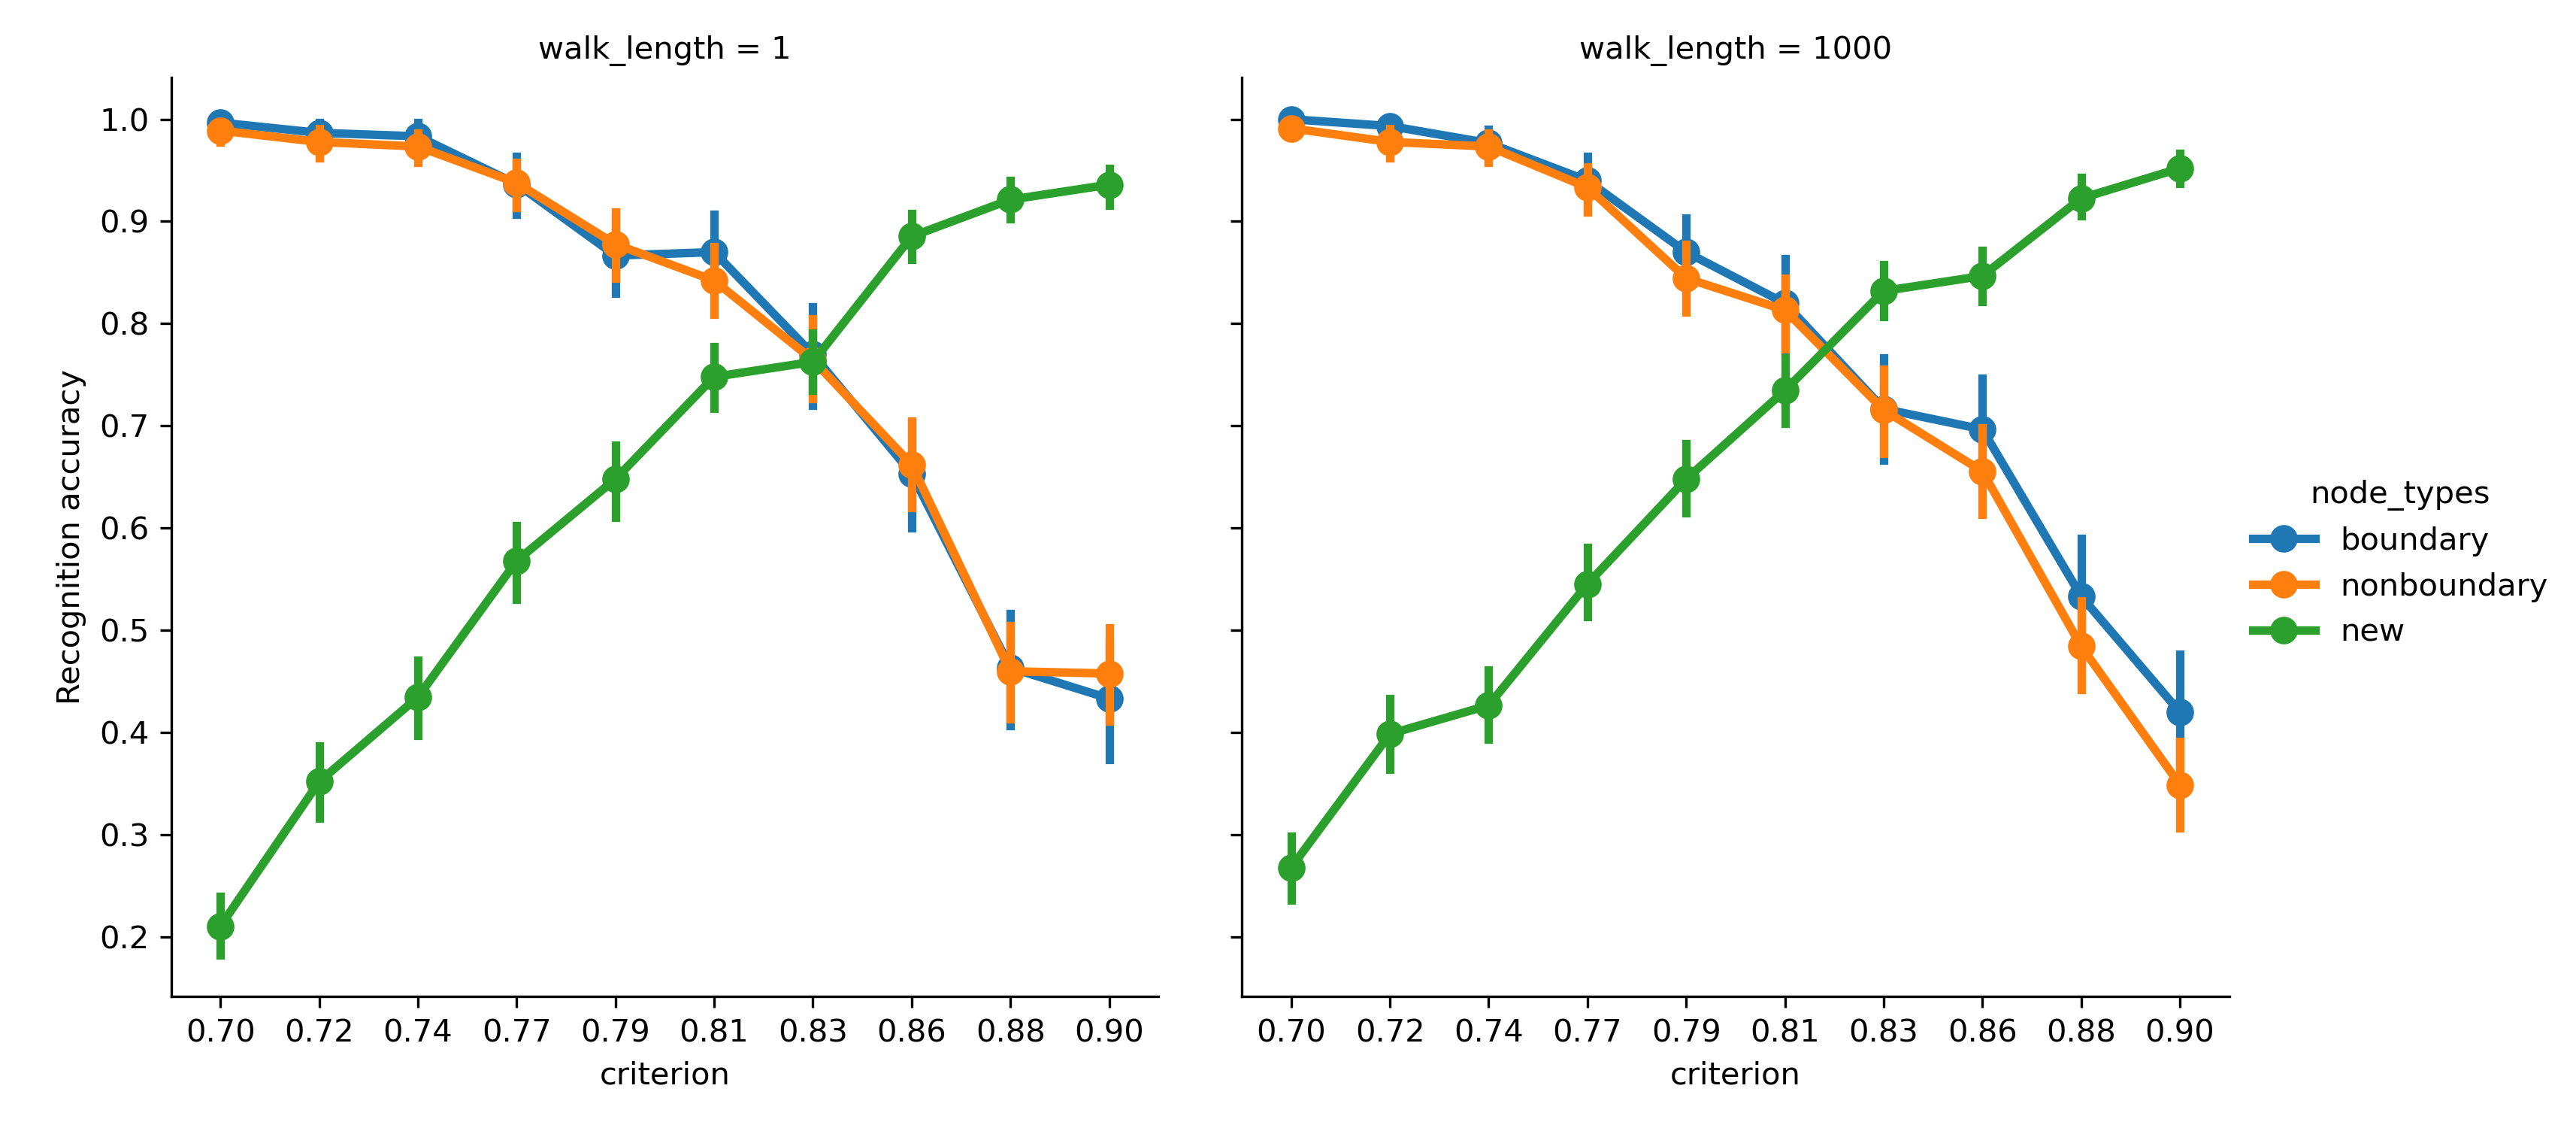
\includegraphics[width = \textwidth]{chapter_notebooks/chapter_3/figures/recog_memory_with_criterion.png}
    \caption{Simulated recognition memory test performances for walk lengths of 1 and walk lengths of 1000 on modular graph in Figure \ref{fig:modular_graph}. On average, recognition memory performance is expected to be better for boundary items than non-boundary items.}
\end{figure}



\section{Methods}
\subsubsection*{Participants}
57 undergraduate students at the University of Massachusetts Amherst participated in this study. Participants were at least 18 years of age and were compensated via course credit. All procedures were approved by the University Institutional Review Board. 

\subsubsection*{Design and Procedures}
Participants were randomly assigned to either a structured exposure or an unstructured exposure group. The overall experimental procedures were the same across both groups. 

Randomly generated polygon shapes were used as stimuli for this experiment. At the beginning of the study, participants were shown 15 polygons which formed the primary stimuli for this study. Participants were asked to carefully study these polygons and to remember their orientation. During 750 exposure trials, separated into 3 blocks of 250, participants were presented these polygons one at a time and asked to judge whether the presented polygon was in its canonical orientation or rotated. Polygons were further surrounded by a (purple, orange, or dark green) colored border.

Each polygon with its border was associated with a node in the three-module graph in figure \ref{fig:modular_graph}. Order of polygons during exposure was determined by a participant's group. The order for 27 participants in the structured exposure group was determined by a random walk through the 3-module graph whereas that for 30 participants in the unstructured group was determined by a random selection among the 15 items (similar to a random walk of length 0). 

\begin{figure}[ht]
    \centering
    \label{fig:exp2-design}
    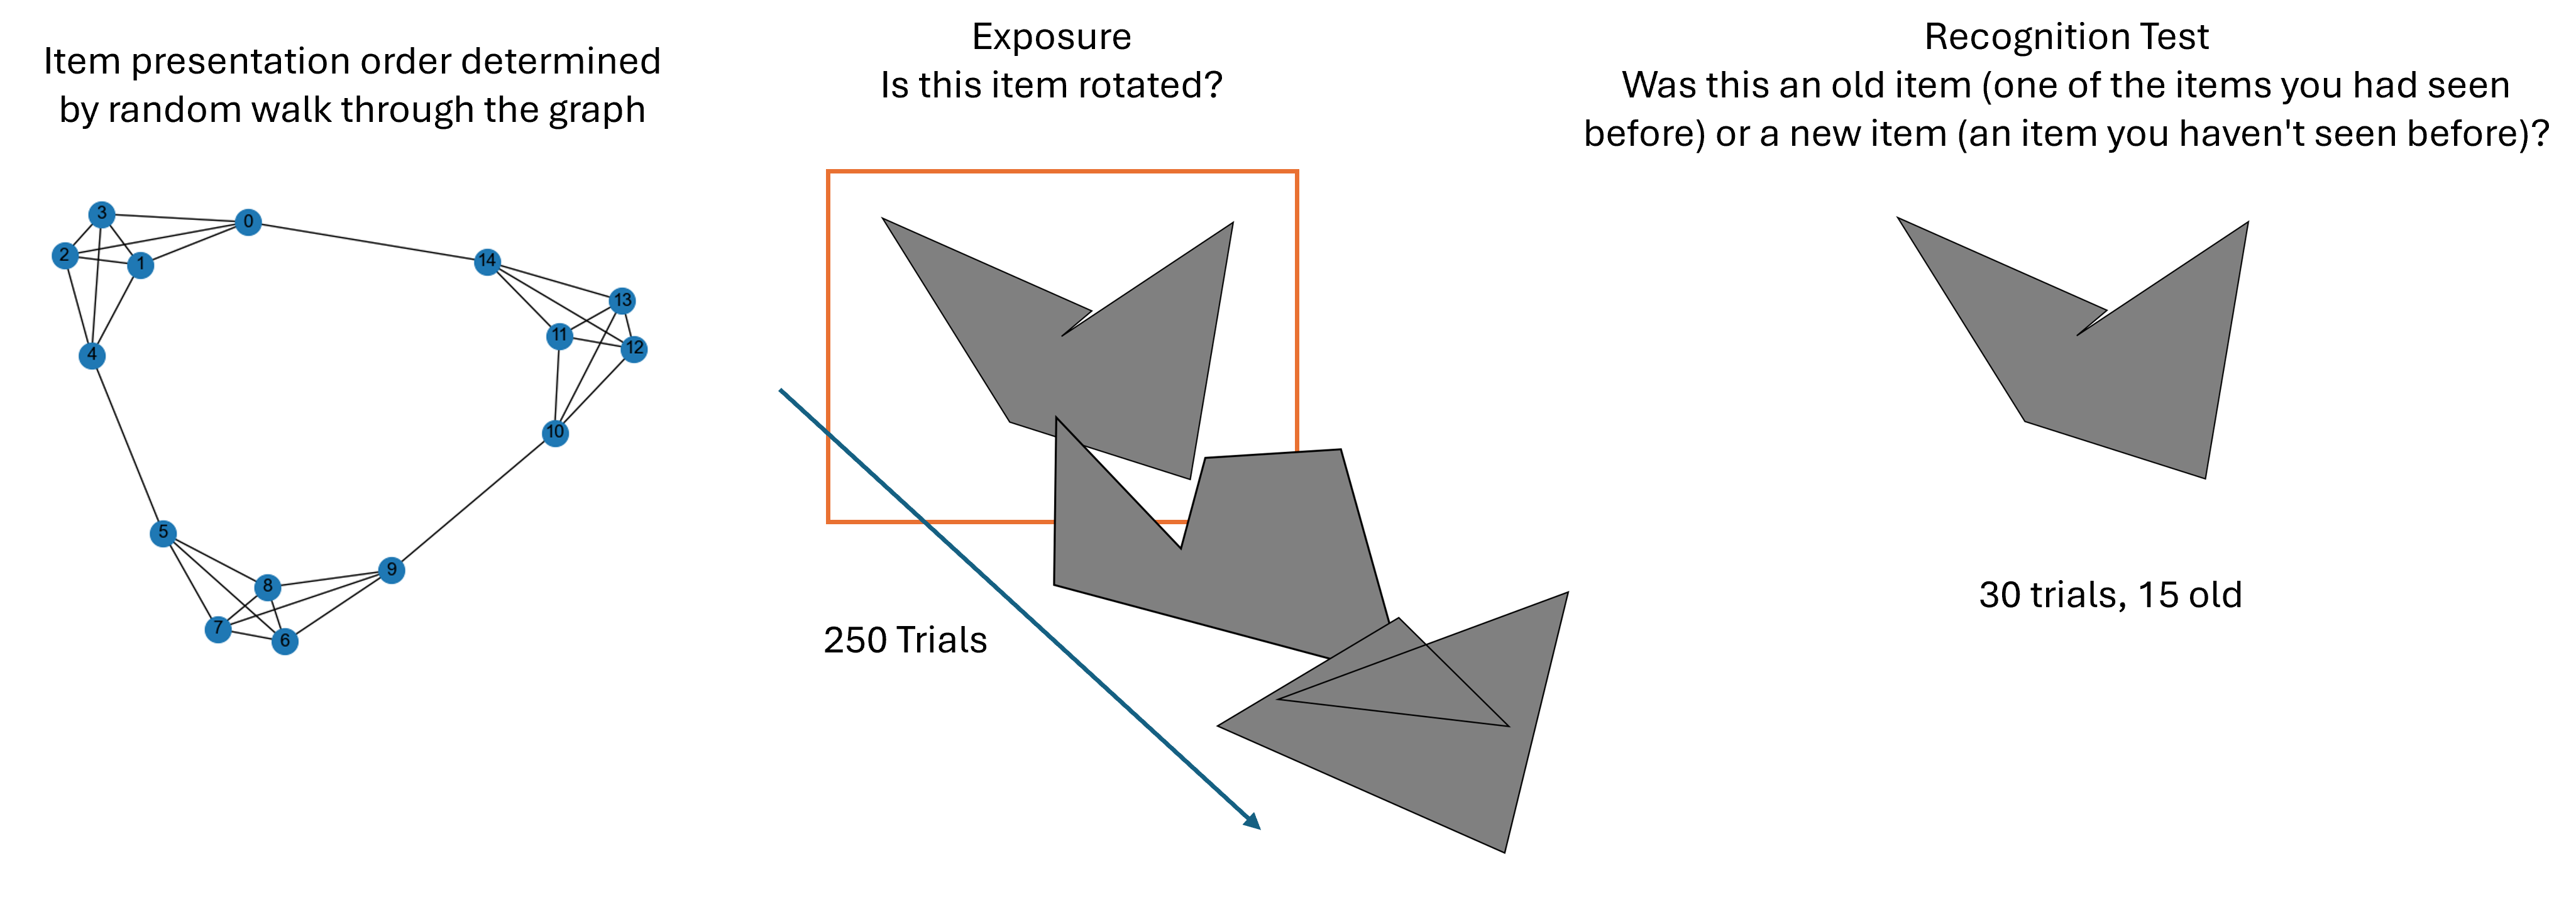
\includegraphics[width = \textwidth]{chapter_notebooks/chapter_3/figures/exp2_design.png}
    \caption{Design schematic for Experiment 2a. Three alternating blocks of exposure and recognition test were presented. A Stroop task was conducted prior to the final recognition test.}
\end{figure}

After each block of the exposure phase, participants went through a recognition memory test (Figure \ref{fig:exp2-design}). They were shown the 15 items they made rotation judgments on (in their canonical orientation) in addition to 15 new random polygon items and were asked to determine whether each of these items was old or new. Order of presentation of old and new items was randomized during the recognition memory test. Of the three recognition tests, the final test was conducted after a short Stroop task to washout any effects of short term memory. 

After the final recognition memory test, participants went through a source memory test. Each of the 15 studied items were shown without the colored borders that surrounded them during exposure. Participants were asked to choose which of the three colored borders, provided as on-screen options, surrounded any particular item. This source memory task was added to provide an additional signal for memory in case of ceiling effects of recognition memory tasks. However, no analyses have been done on this source memory task. 


\section{Results}
Table \ref{tab:exp2-rt-accuracy-stats} provides the means and standard deviations for response times and accuracies across each block for all stimuli types for both conditions. 
\begin{table}
    \centering
    \label{tab:exp2-rt-accuracy-stats}
    \caption{Accuracy and Response time Means and Standard Deviations for exposure and recognition phases in experiment 2}    
    \begin{tabular}{llllrrrr}
        \toprule
         &  &  &  & \multicolumn{2}{r}{accuracy} & \multicolumn{2}{r}{rt} \\
         &  &  &  & mean & std & mean & std \\
        phase & block & stimulus type & condition &  &  &  &  \\
        \midrule
        \multirow[t]{12}{*}{exposure} & \multirow[t]{4}{*}{0} & \multirow[t]{2}{*}{boundary} & structured & 0.683 & 0.465 & 1.644 & 1.911 \\
         &  &  & unstructured & 0.739 & 0.439 & 1.710 & 1.732 \\
        \cline{3-8}
         &  & \multirow[t]{2}{*}{nonboundary} & structured & 0.669 & 0.471 & 1.619 & 1.728 \\
         &  &  & unstructured & 0.728 & 0.445 & 1.713 & 1.689 \\
        \cline{2-8} \cline{3-8}
         & \multirow[t]{4}{*}{1} & \multirow[t]{2}{*}{boundary} & structured & 0.735 & 0.441 & 1.244 & 1.322 \\
         &  &  & unstructured & 0.796 & 0.403 & 1.283 & 1.243 \\
        \cline{3-8}
         &  & \multirow[t]{2}{*}{nonboundary} & structured & 0.739 & 0.439 & 1.250 & 1.343 \\
         &  &  & unstructured & 0.790 & 0.408 & 1.263 & 1.217 \\
        \cline{2-8} \cline{3-8}
         & \multirow[t]{4}{*}{2} & \multirow[t]{2}{*}{boundary} & structured & 0.757 & 0.429 & 1.168 & 1.657 \\
         &  &  & unstructured & 0.843 & 0.363 & 1.111 & 1.334 \\
        \cline{3-8}
         &  & \multirow[t]{2}{*}{nonboundary} & structured & 0.765 & 0.424 & 1.192 & 1.656 \\
         &  &  & unstructured & 0.838 & 0.369 & 1.085 & 1.546 \\
        \cline{1-8} \cline{2-8} \cline{3-8}
        \multirow[t]{18}{*}{memory} & \multirow[t]{6}{*}{0} & \multirow[t]{2}{*}{boundary} & structured & 0.796 & 0.404 & 1.681 & 1.490 \\
         &  &  & unstructured & 0.878 & 0.328 & 1.805 & 1.712 \\
        \cline{3-8}
         &  & \multirow[t]{2}{*}{new} & structured & 0.721 & 0.449 & 1.899 & 1.569 \\
         &  &  & unstructured & 0.782 & 0.413 & 1.770 & 1.666 \\
        \cline{3-8}
         &  & \multirow[t]{2}{*}{nonboundary} & structured & 0.782 & 0.414 & 1.715 & 1.602 \\
         &  &  & unstructured & 0.904 & 0.296 & 1.570 & 1.291 \\
        \cline{2-8} \cline{3-8}
         & \multirow[t]{6}{*}{1} & \multirow[t]{2}{*}{boundary} & structured & 0.833 & 0.374 & 1.564 & 2.573 \\
         &  &  & unstructured & 0.911 & 0.285 & 1.212 & 0.959 \\
        \cline{3-8}
         &  & \multirow[t]{2}{*}{new} & structured & 0.800 & 0.400 & 1.420 & 1.486 \\
         &  &  & unstructured & 0.873 & 0.333 & 1.338 & 1.056 \\
        \cline{3-8}
         &  & \multirow[t]{2}{*}{nonboundary} & structured & 0.860 & 0.348 & 1.618 & 1.812 \\
         &  &  & unstructured & 0.874 & 0.332 & 1.139 & 0.709 \\
        \cline{2-8} \cline{3-8}
         & \multirow[t]{6}{*}{2} & \multirow[t]{2}{*}{boundary} & structured & 0.907 & 0.291 & 1.196 & 1.194 \\
         &  &  & unstructured & 0.900 & 0.301 & 1.075 & 0.694 \\
        \cline{3-8}
         &  & \multirow[t]{2}{*}{new} & structured & 0.751 & 0.433 & 1.454 & 2.322 \\
         &  &  & unstructured & 0.844 & 0.363 & 1.292 & 1.127 \\
        \cline{3-8}
         &  & \multirow[t]{2}{*}{nonboundary} & structured & 0.893 & 0.310 & 1.370 & 1.869 \\
         &  &  & unstructured & 0.926 & 0.262 & 1.045 & 0.729 \\
        \cline{1-8} \cline{2-8} \cline{3-8}
        \bottomrule
        \end{tabular}
    \end{table}
        
As expected, accuracies for old stimuli increase with increased exposure (Figure \ref{fig:exp2-accuracies}) wheras the response times decreased with more experience with the stimuli across blocks (Figure\ref{fig:exp2-rts}). \footnote{Interestingly, overall accuracy of participants in the unstructured exposure condition is higher, than those in the structured exposure condition across all stimulus types. This effect may be due to participant variability.} 

\begin{figure}
    \centering
    \label{fig:exp2-accuracies}
    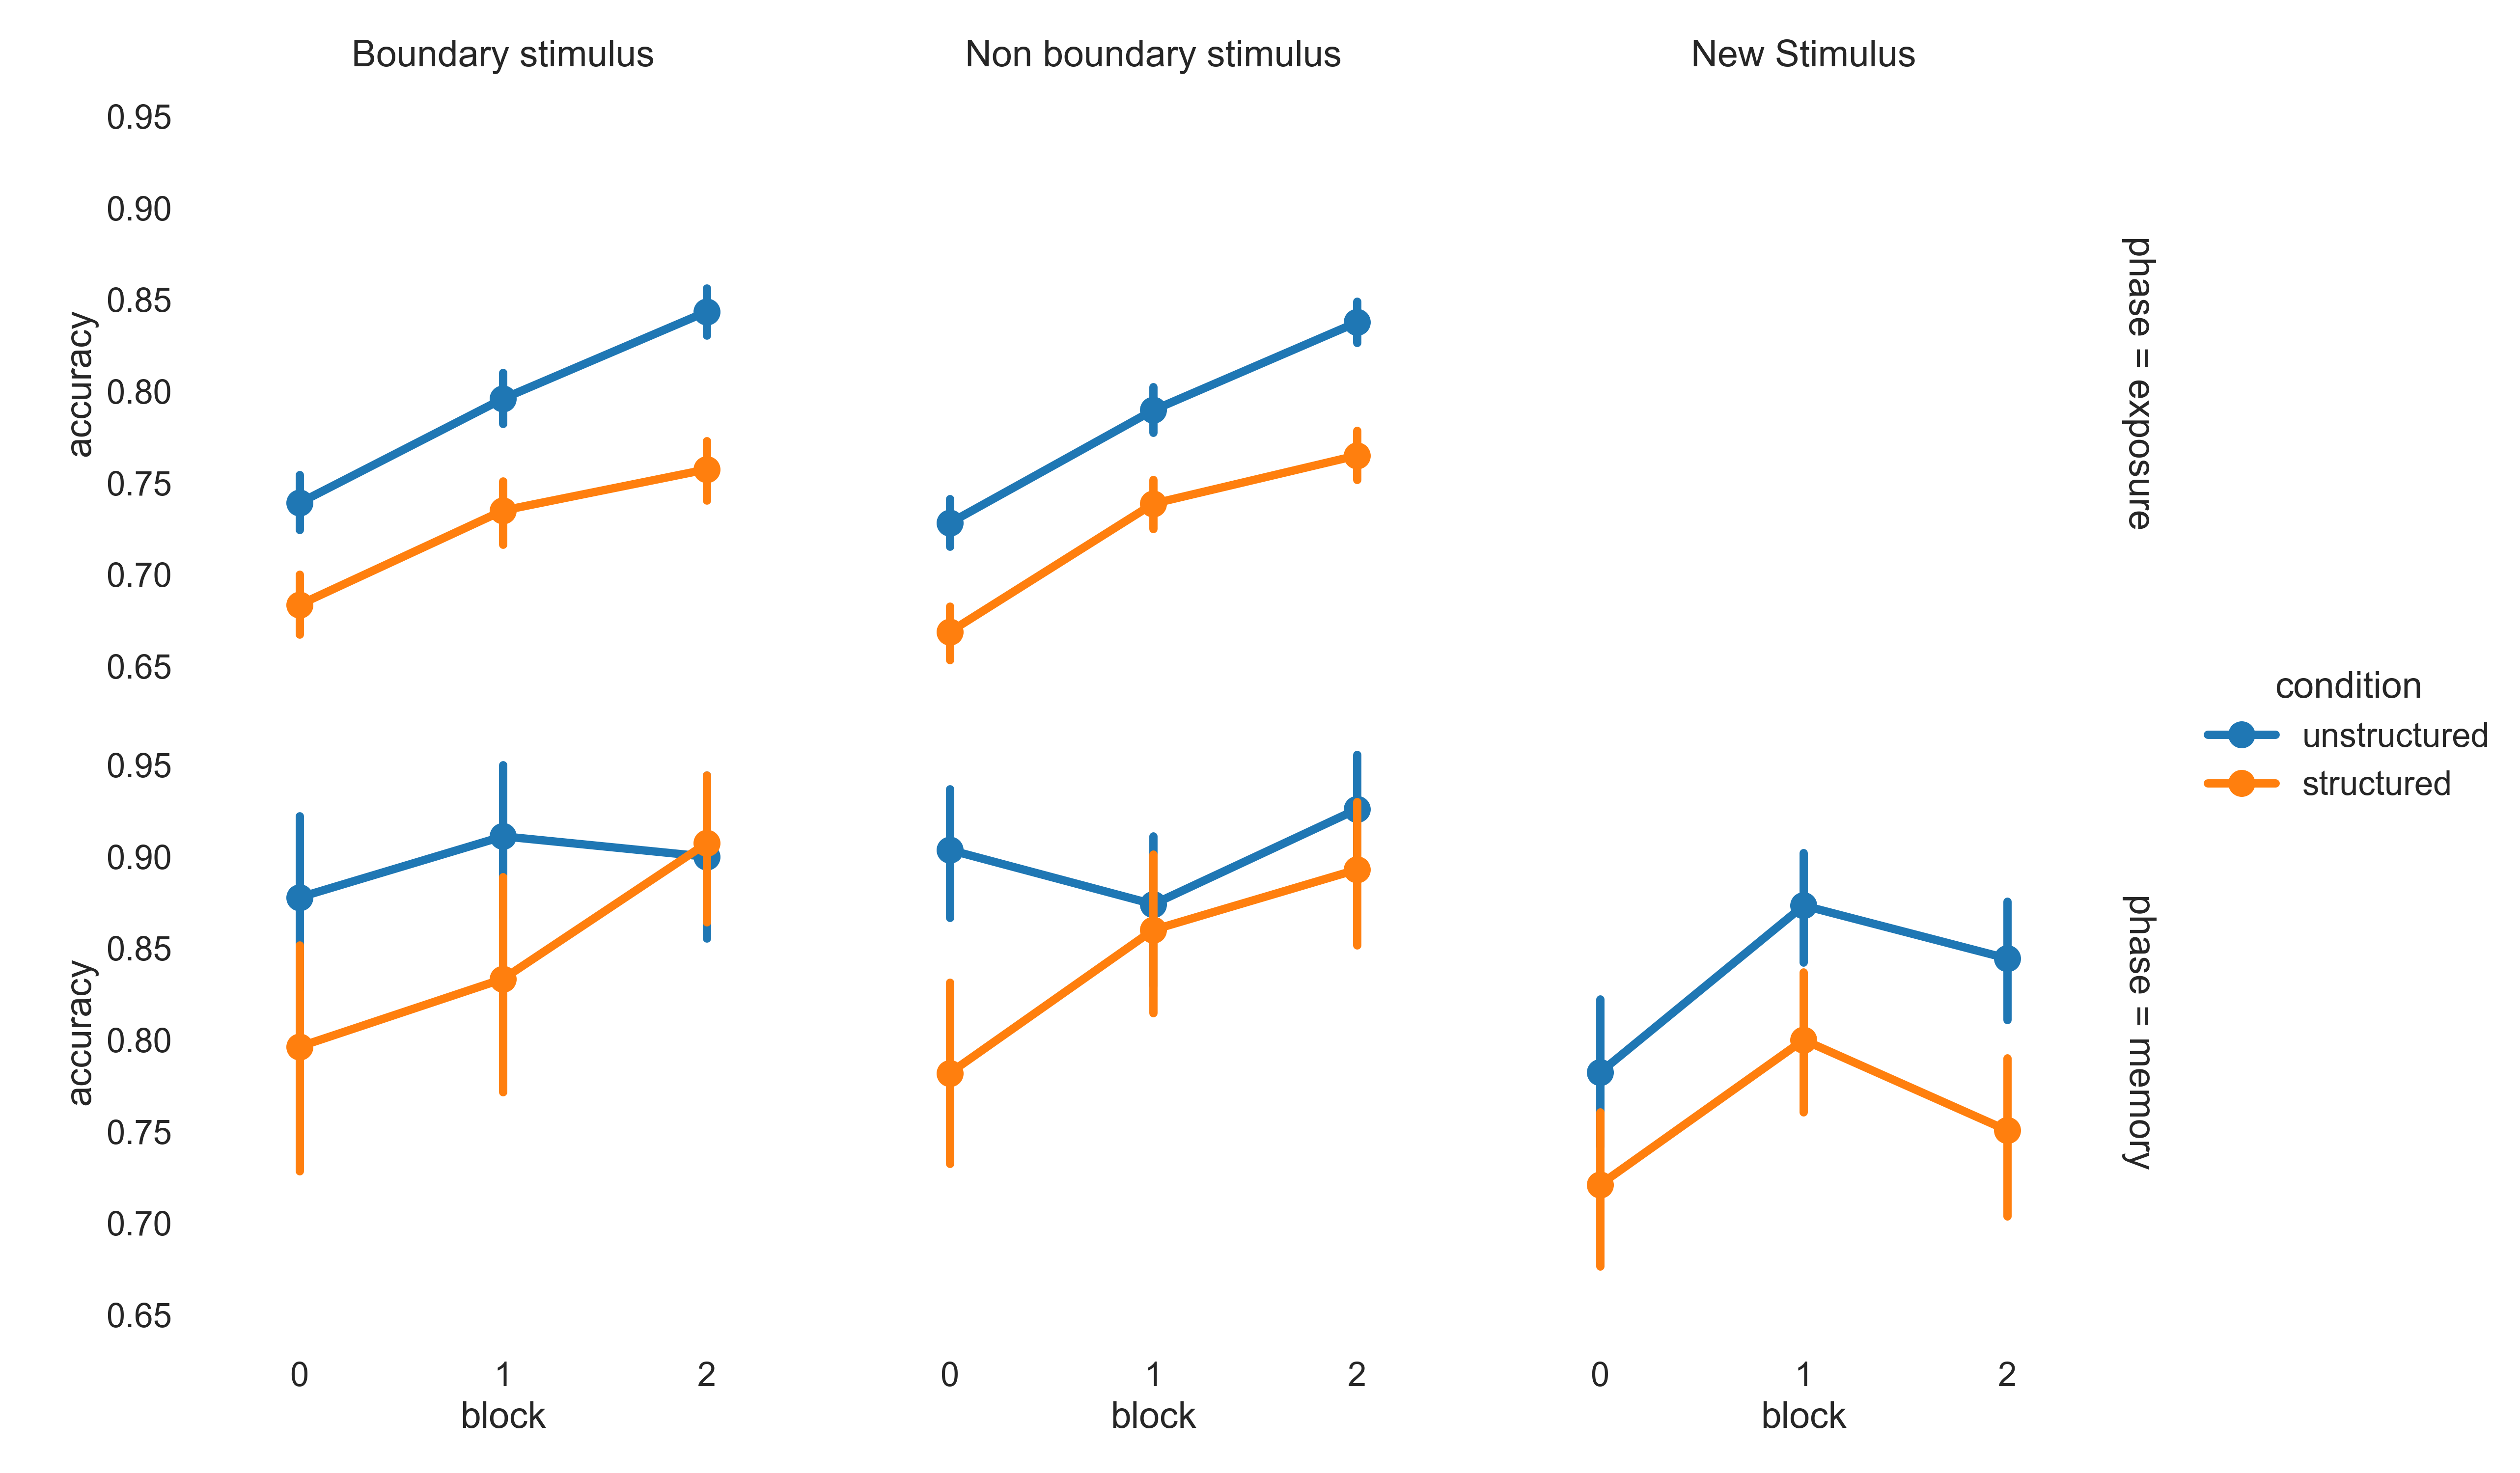
\includegraphics[width = \textwidth]{chapter_notebooks/chapter_3/figures/exposure_recog_accuracy_allphases.png}
    \caption{Mean accuracies for both participant groups (structured and unstructured) across blocks, for different stimulus types and phases of the experiment}
\end{figure}


\begin{figure}
    \centering
    \label{fig:exp2-rts}
    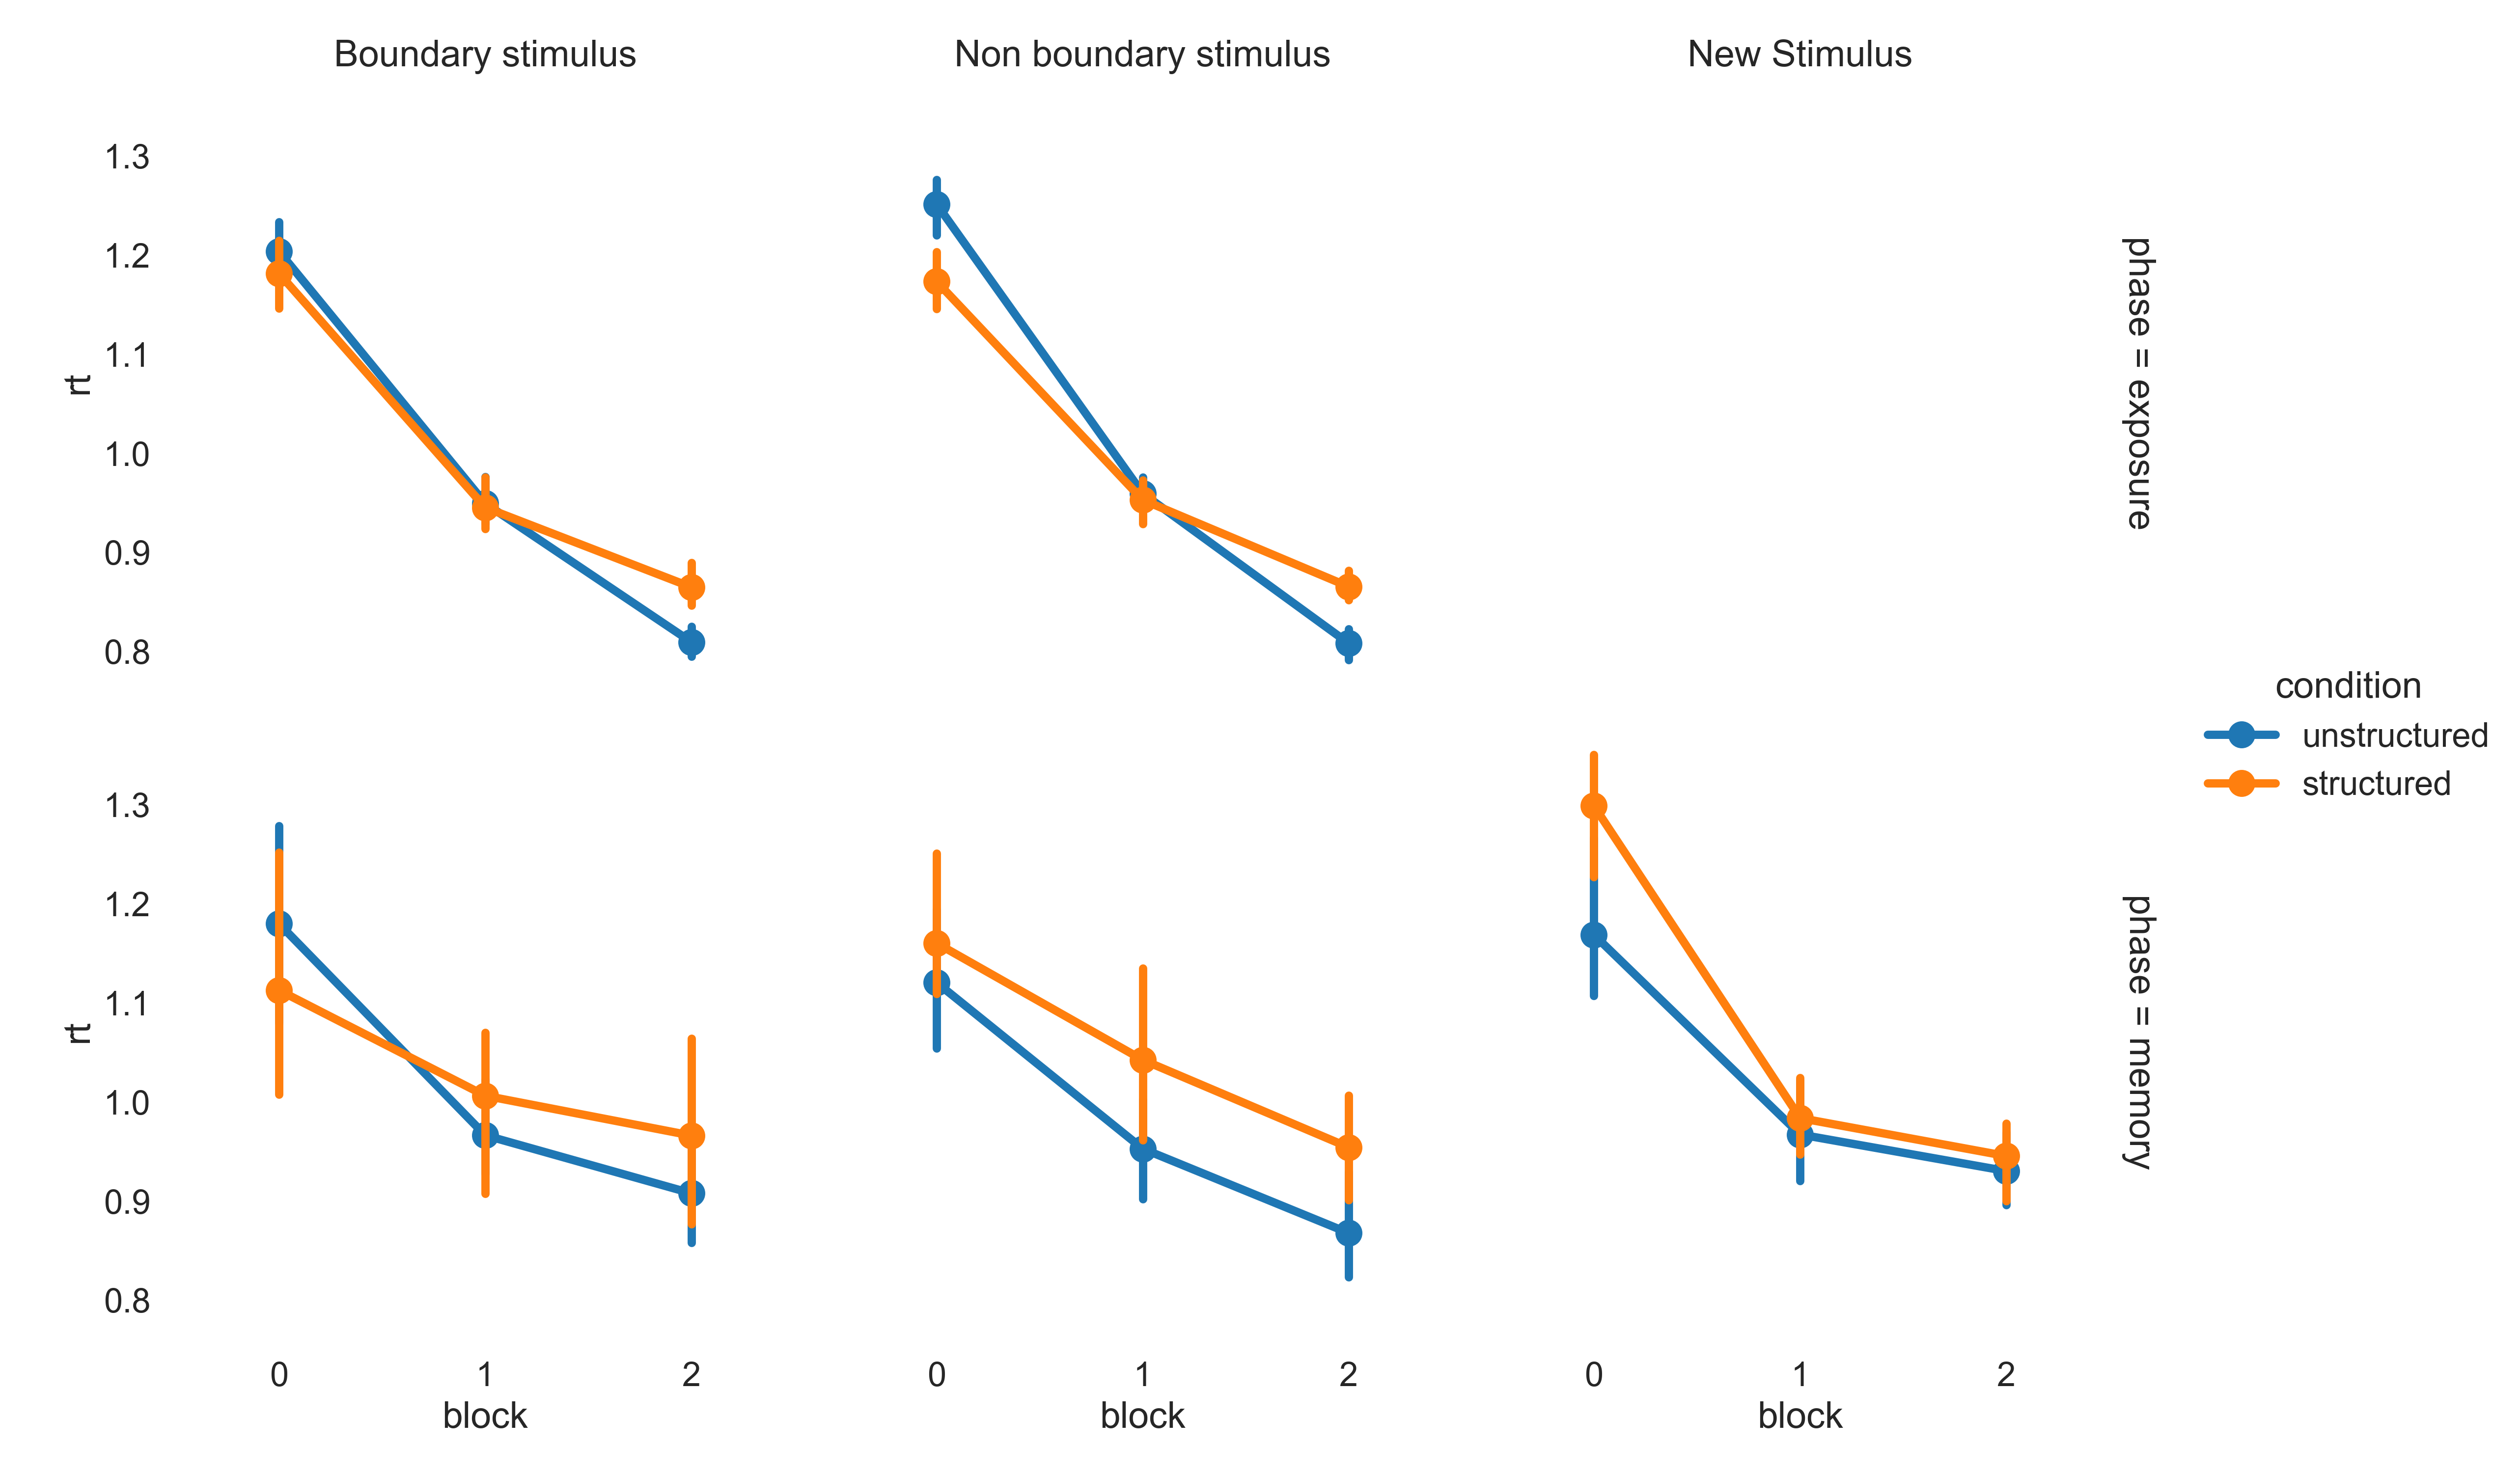
\includegraphics[width = \textwidth]{chapter_notebooks/chapter_3/figures/exposure_recog_rt_allphases.png}
    \caption{Median response times for both participant groups (structured and unstructured) across blocks, for different stimulus types and phases of the experiment}
\end{figure}

To assess differences between stimulus types (boundary vs non boundary) on recognition memory, a signal detection (SDT) model was first fit separately for boundary and non boundary items. The model for boundary items describes the probability of responding `old' to old boundary stimuli relative to new stimuli. Similarly, the model for non boundary items describes the probability of responding `old' to old non-boundary items relative to new stimuli. A participant intercept term allows for each participant to have their own decision criterion. Finally, accuracy at exposure was included as a factor in the SDT model. Exposure accuracy factor for old items was computed by averaging the rotation judgment accuracy for each of the old items in the block immediately before the recognition memory block. For new items, this factor was computed by averaging the rotation judgment accuracy for all exposure items in the exposure block before that recognition phase. The model fits relatively well as shown in figure \ref{fig:exp2-sdt-fits}.

\begin{figure}
    \centering
    \label{fig:exp2-sdt-fits}
    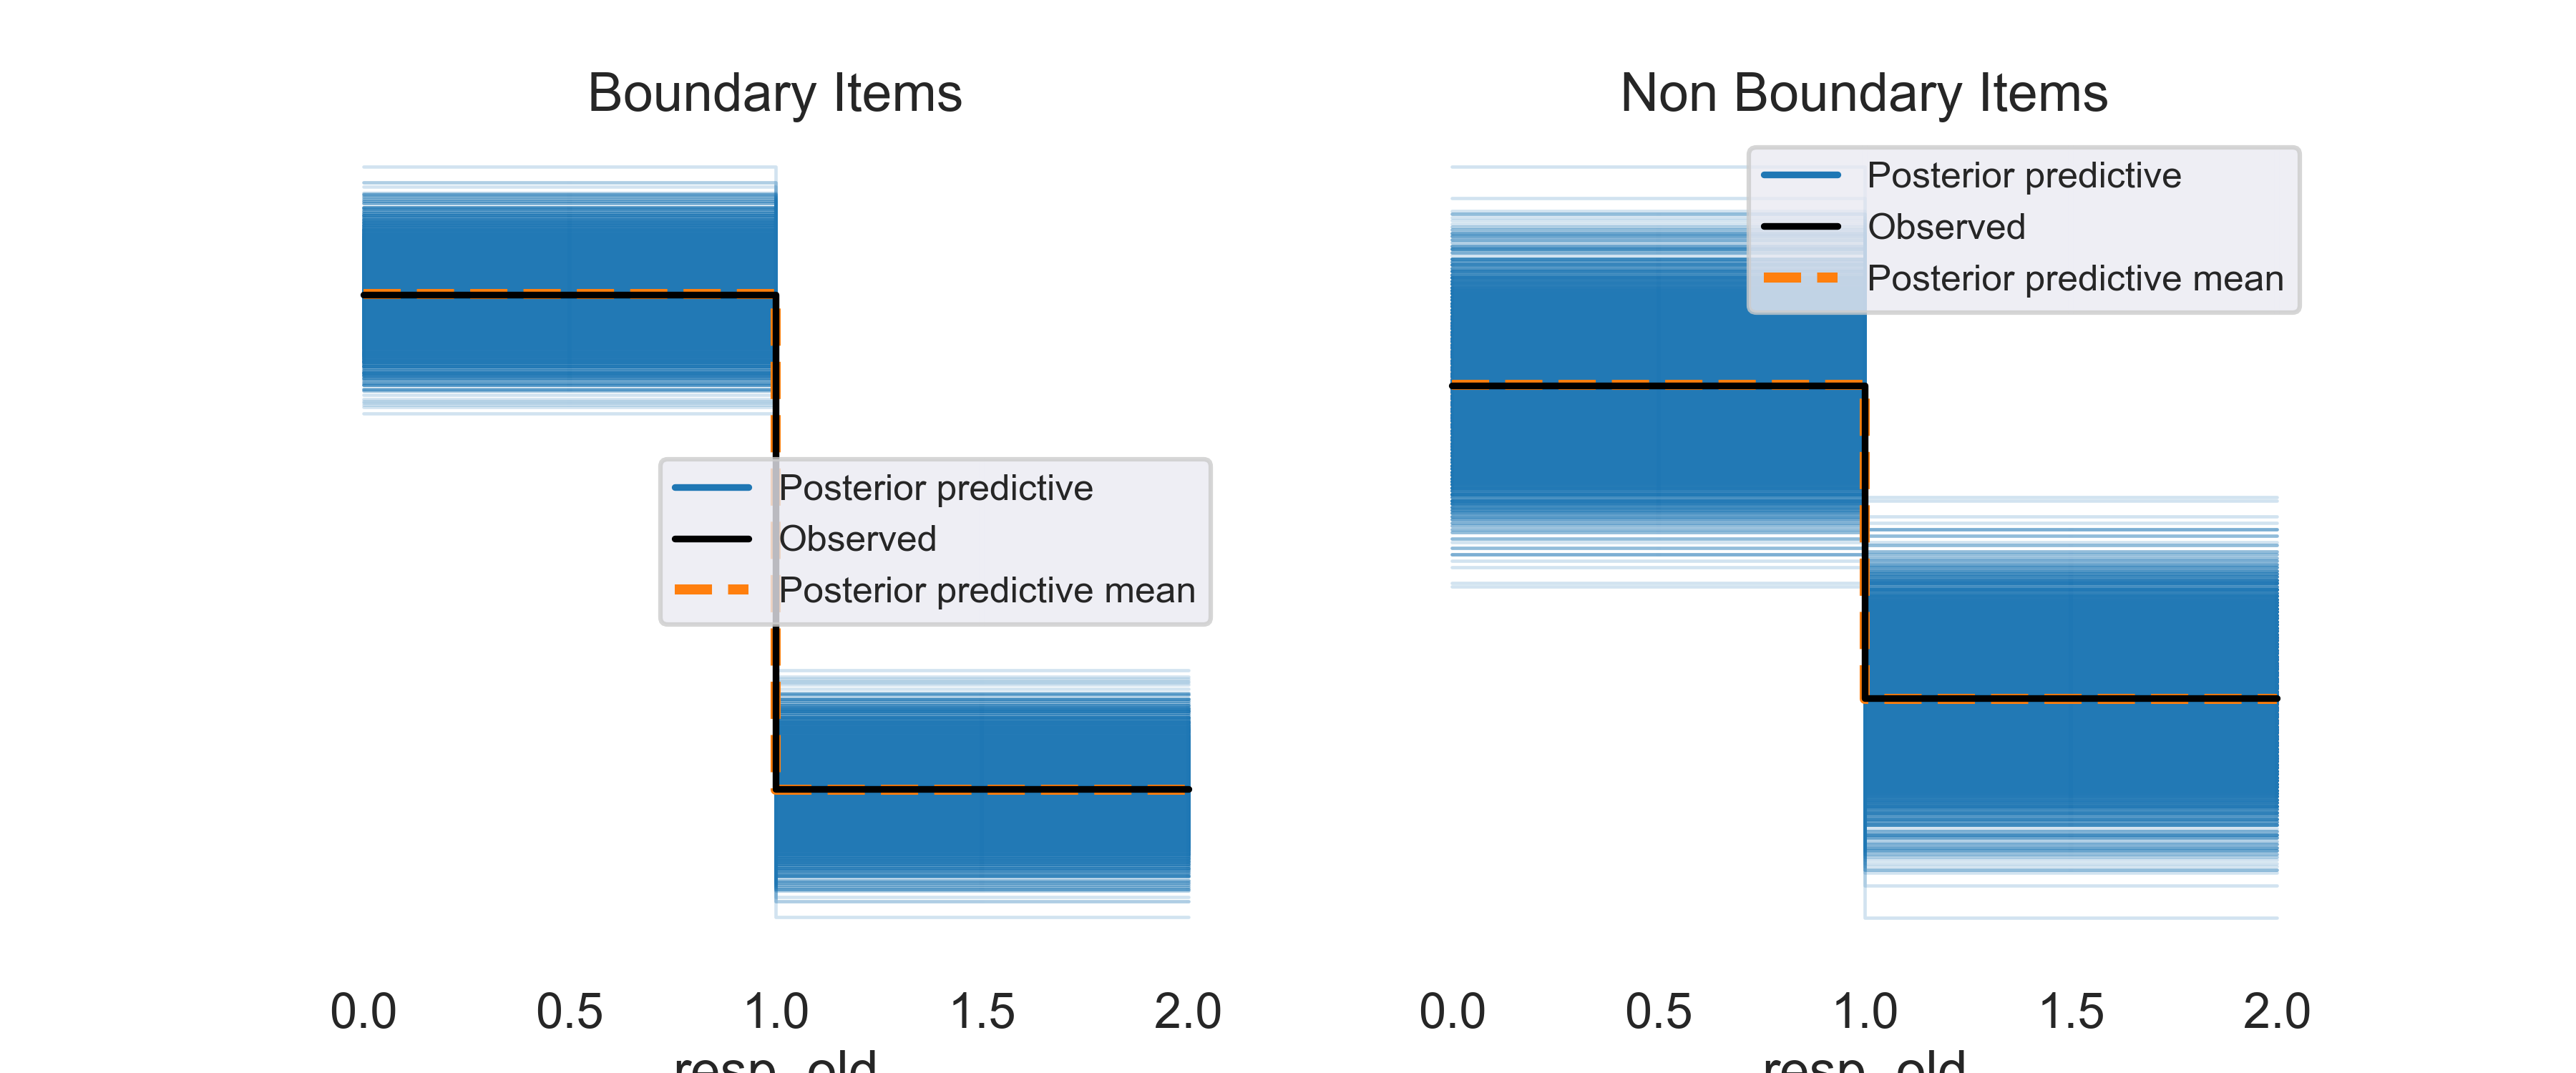
\includegraphics[width = \textwidth]{chapter_notebooks/chapter_3/figures/ppc_sdt_model.png}
    \caption{SDT Model Posterior Predictive Distributions for boundary and non boundary items}
\end{figure}

$d'$ measures the distance between distributions of old and new items. Parameter estimates of $d'$ for structured relative to unstructured for boundary and non boundary nodes for the final recognition block are shown in figure \ref{fig:sdt-params}. Parameter statistics are reported in appendix tables \ref{tab:exp3-bayesmodel-boundary-sdt} and \ref{tab:exp3-bayesmodel-nonboundary-sdt}

\begin{figure}
    \centering
    \label{fig:sdt-params}
    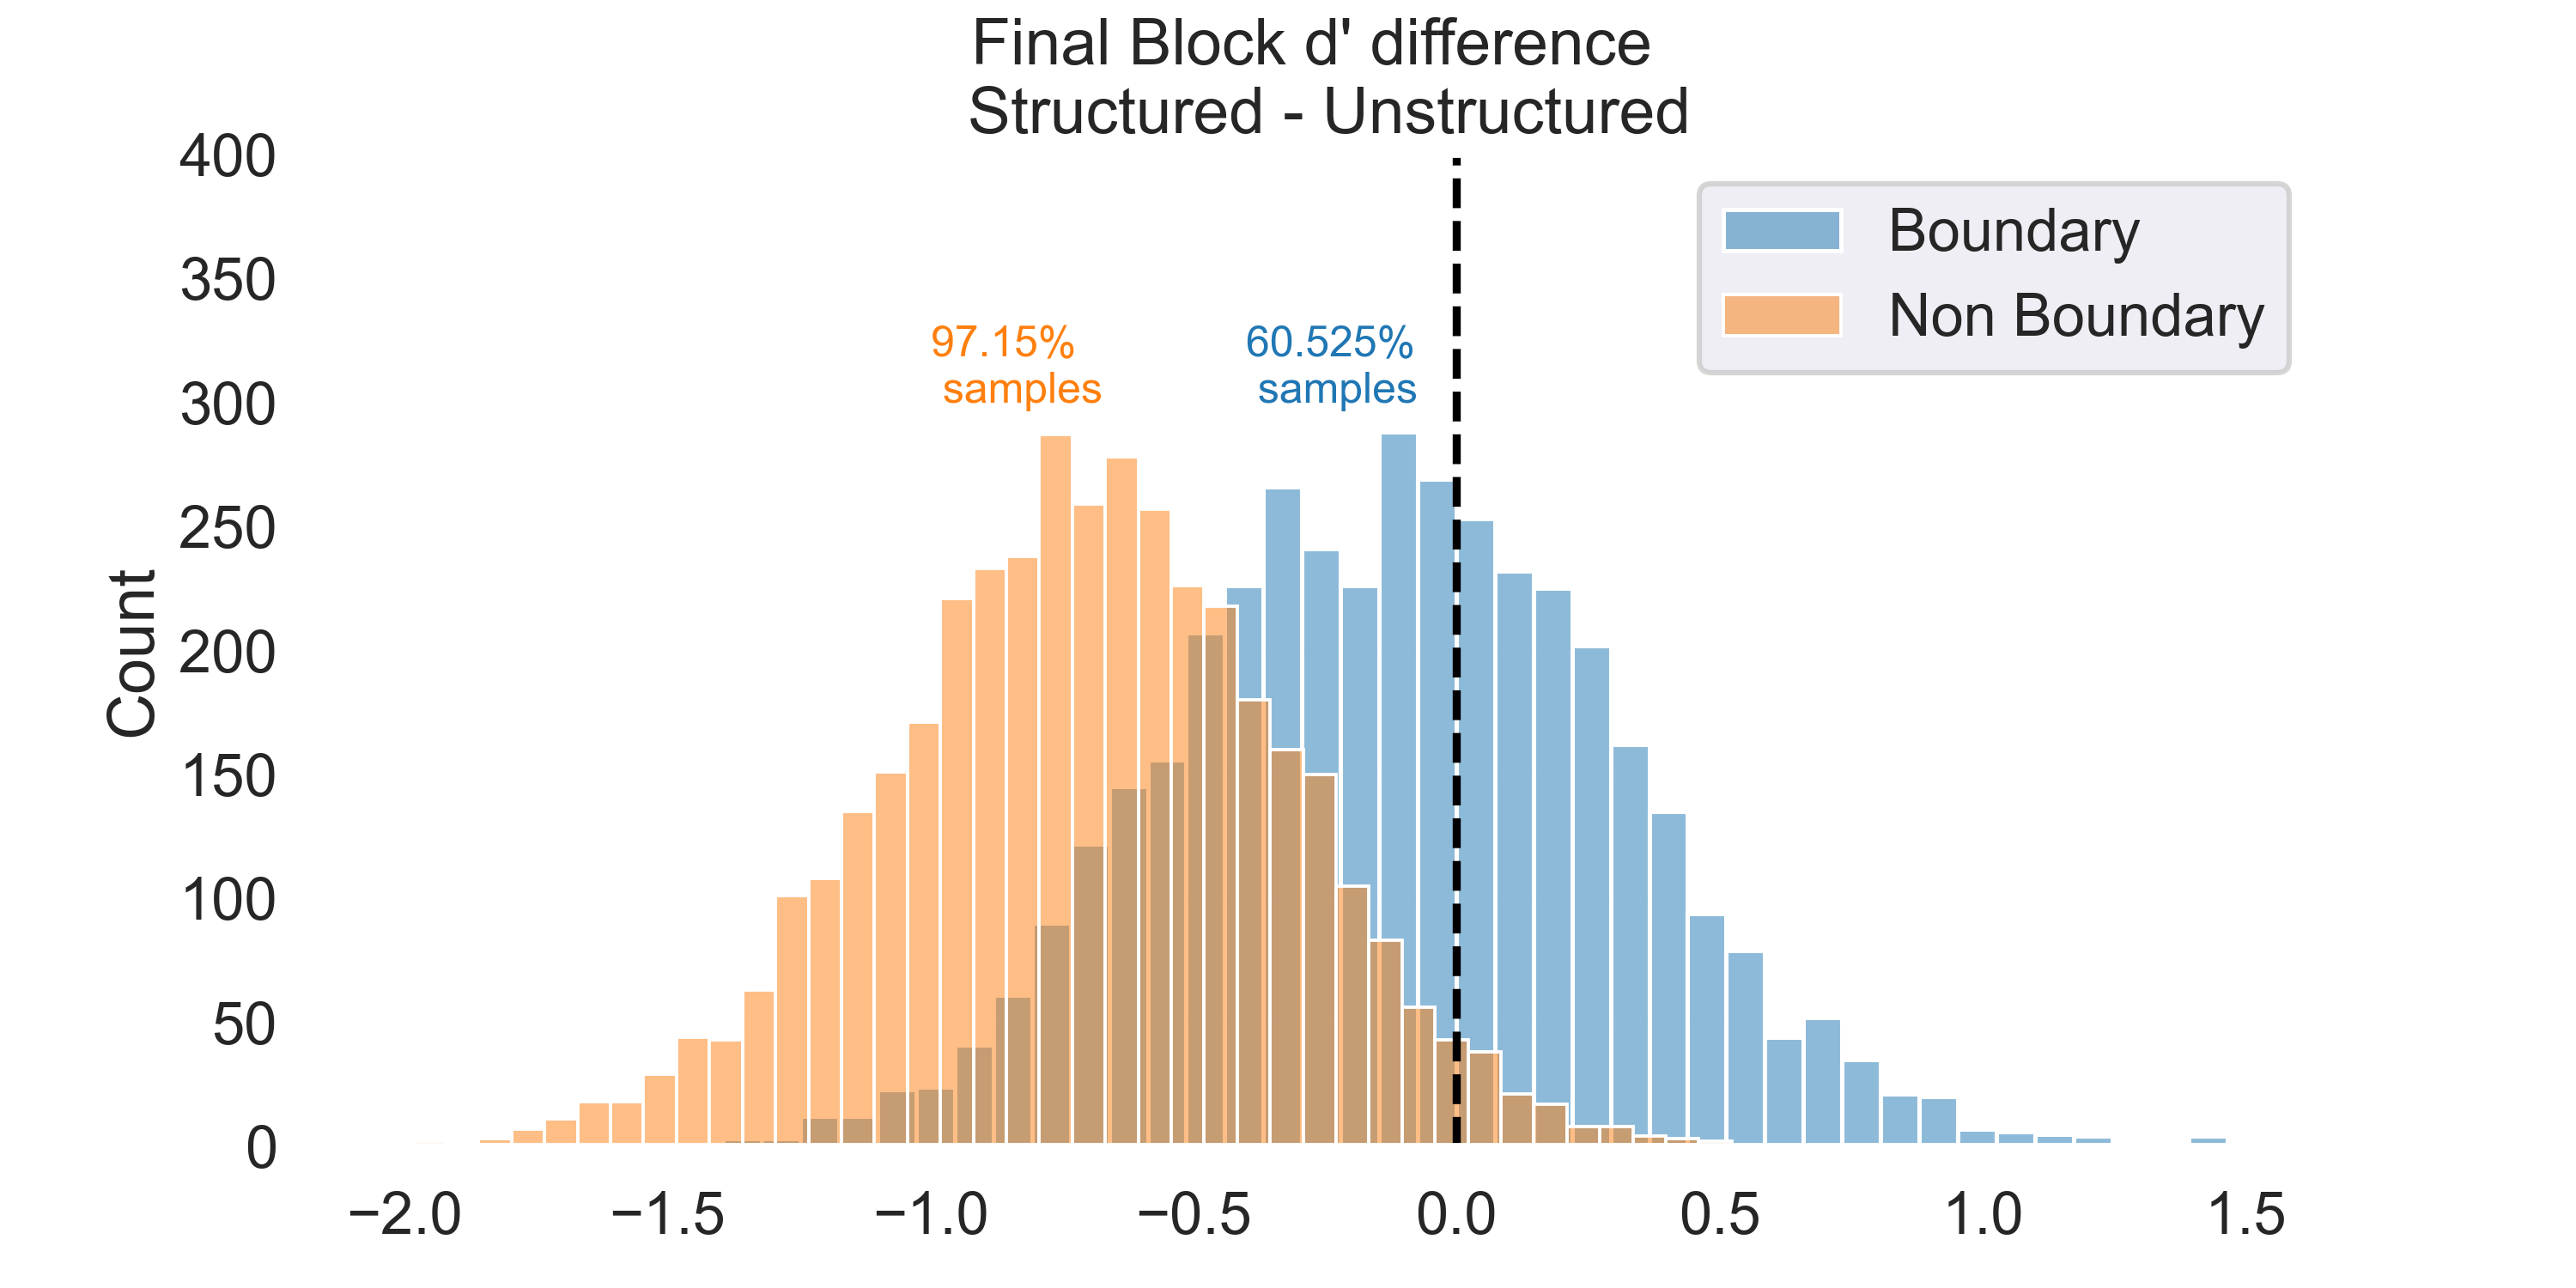
\includegraphics[width = \textwidth]{chapter_notebooks/chapter_3/figures/sdt_d_results.png}
    \caption{Differences in $d'$ for models fit to separately boundary and non boundary nodes for both structured and unstructured exposure conditions}
\end{figure}

The SDT modeling implies that while there are no differences in recognition memory for boundary nodes based on exposure, non boundary nodes become less recognizable under structured exposure condition. However, 

\subsection*{Diffusion Modeling}
However, the model used above fails to account for ceiling effects -- accuracy for old items is near perfect or could have reached an asymptote. Those models also do not account for encoding accuracy during exposure -- participants may fail to recognize old items if they did not study those items well as indicated by the rotation judgement task. Models were also fit separately to derive $d'$ for boundary and non-boundary items, thus losing shared variability within the participant.

To be able to account for both ceiling effects and effects of exposure, we can use additional information available in form of response times during the recognition memory task. For example, for participants equally accurate in recognizing boundary and non-boundary participants, being able to recognize boundary items faster may provide additional evidence for better memorability of these items relative to slower recognized non-boundary items. Figure \ref{fig:recognition-rts} shows median response times across three blocks of recognition test. 

To understand recognition memory differences between boundary and non-boundary items in context of response accuracy and response time distributions, we use the Drift Diffusion Model \(DDM\). The DDM, which falls under a class of sequential sampling models, has been a widely successful model in modeling two-choice tasks in recognition memory \cite{ratcliff2004diffusion, ratcliff2022discriminating, starns2014using, starns2014validating, ratcliff2009modeling}. The function of the DDM is depicted in Figure \ref{fig:ddm-model}. 

\begin{figure}[ht]
    \label{fig:ddm-model}
    \centering
    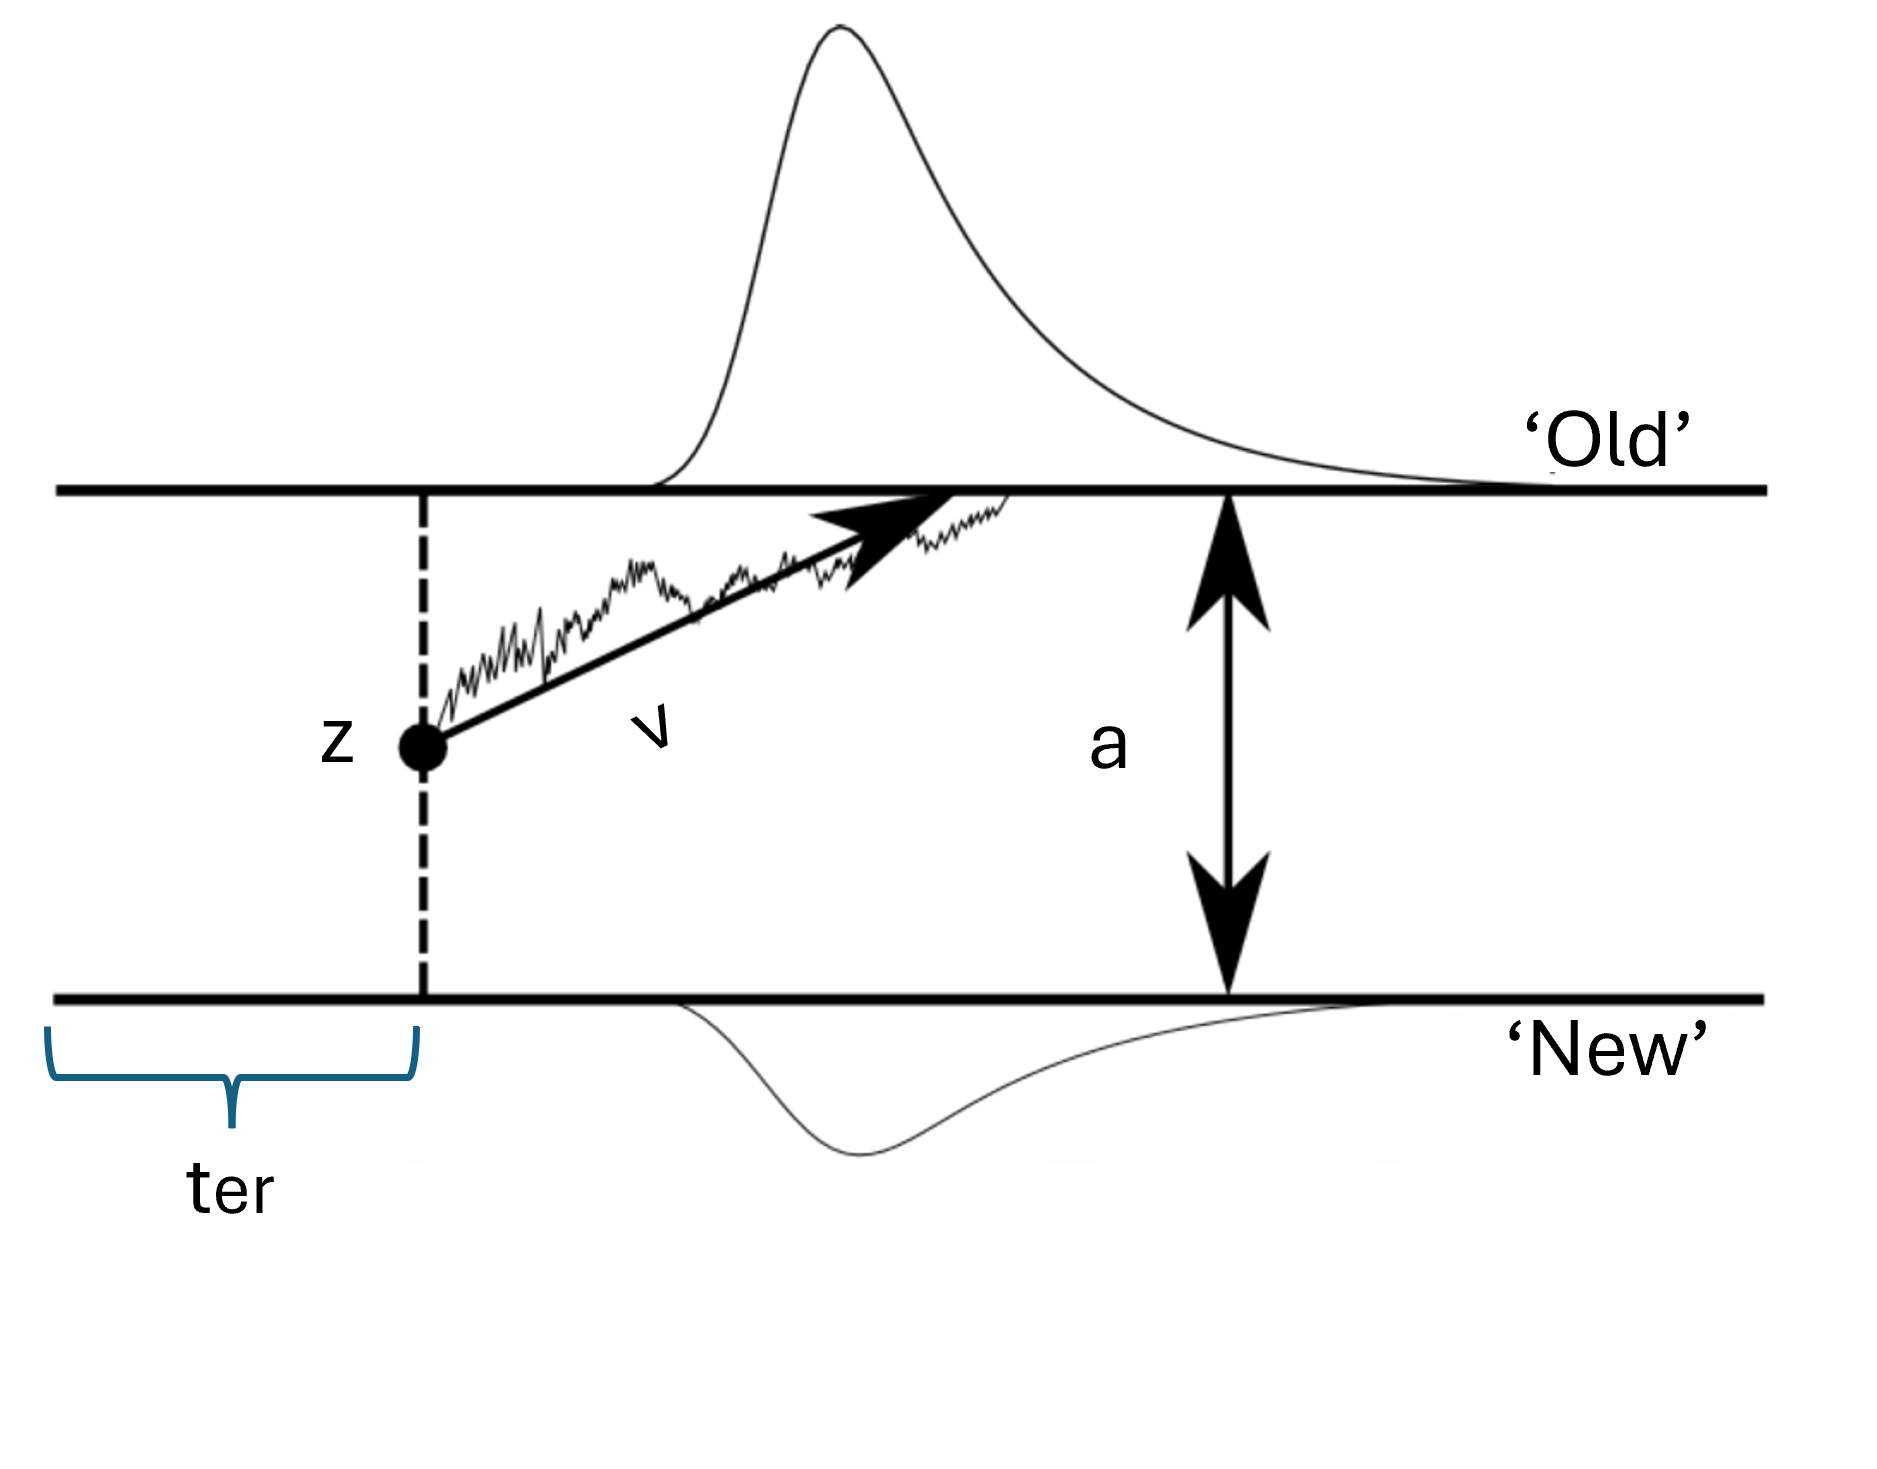
\includegraphics[width = 0.75\textwidth]{chapter_notebooks/chapter_3/figures/ddm.png}
    \caption{The Drift Diffusion Model of Choice Response Times for Old/New recognition memory tasks.}
\end{figure}

Briefly, the DDM assumes that at choice time, evidence from two presented options accumulates sequentially over time towards one of the two boundaries. For a previously studied item presented at test, the evidence from the item accumulates slowly towards the `old' boundary whereas for a non-studied item, the evidence accumulates towards the `new' boundary. The rate of evidence accumulation is controlled by the drift rate parameter, `$v$'. Participants may be biased towards making an old or a new response at test; this bias is measured by the starting point parameter, `$z$'. THe boundary separation between the two responses is modeled by a parameter `$a$'. Finally, the observed response consists of cognitive processes not affiliated with decision making (such as time it takes to visually process the test item, time for the motor systems to click the relevant key) which are modeled by a non-decision time parameter `$t_{er}$'. \footnote{Note that this version of the DDM is a simplified model. More complex DDMs account for trial-to-trial variability in each parameters as well.} 

Prior work has shown that memory strength of previously studied items impacts the drift rate towards old/new responses. The drift rate parameter implies that a stronger match to memory leads to a quicker accumulation of evidence towards the `old' response boundary. Similarly, a stronger mis-match to memory allows for a quicker accumulation of evidence towards the `new' response boundary\cite{ratcliff2004diffusion,ratcliff2022discriminating}. 

The DDM thus allows us circumvent ceiling effects by modeling response time distributions and estimate whether if boundary items are indeed a remembered better than non-boundary items in the structured exposure or whether the effect is driven by worse-remembered non-boundary items. 

For the recognition task in the current study, the DDM was parameterized as follows: 
\begin{equation}
    \begin{aligned}
        v \sim 0 + node type:condition:block + accuracy exposure \\
        z \sim 0 + block \\
        a \sim 0 + condition:block \\
        t = 0.25
    \end{aligned}
\end{equation}

The fixed value of the non decision time parameter $t$ was derived by first fitting the DDM over a range of possible $t$ values (i.e. a grid search) and picking value with the best fitting model in that range. DDM models were fit using the HSSM package \cite{fengler2022beyond}. \footnote{Unfortunately the non decision time parameter is too difficult to fit -- this is a known problem with the HSSM package} 

\subsubsection*{DDM Results}
The modeling framework above allows incorporating response times during recognition memory tasks. In particular, if an item has quickly and accurately recognized as old or new, in addition to good accuracy, such recognition would result into faster reaction times. This effect is captured by the drift rate parameter of the DDM. 

\begin{figure}
    \centering
    \label{fig:ddm-drift-rates}
    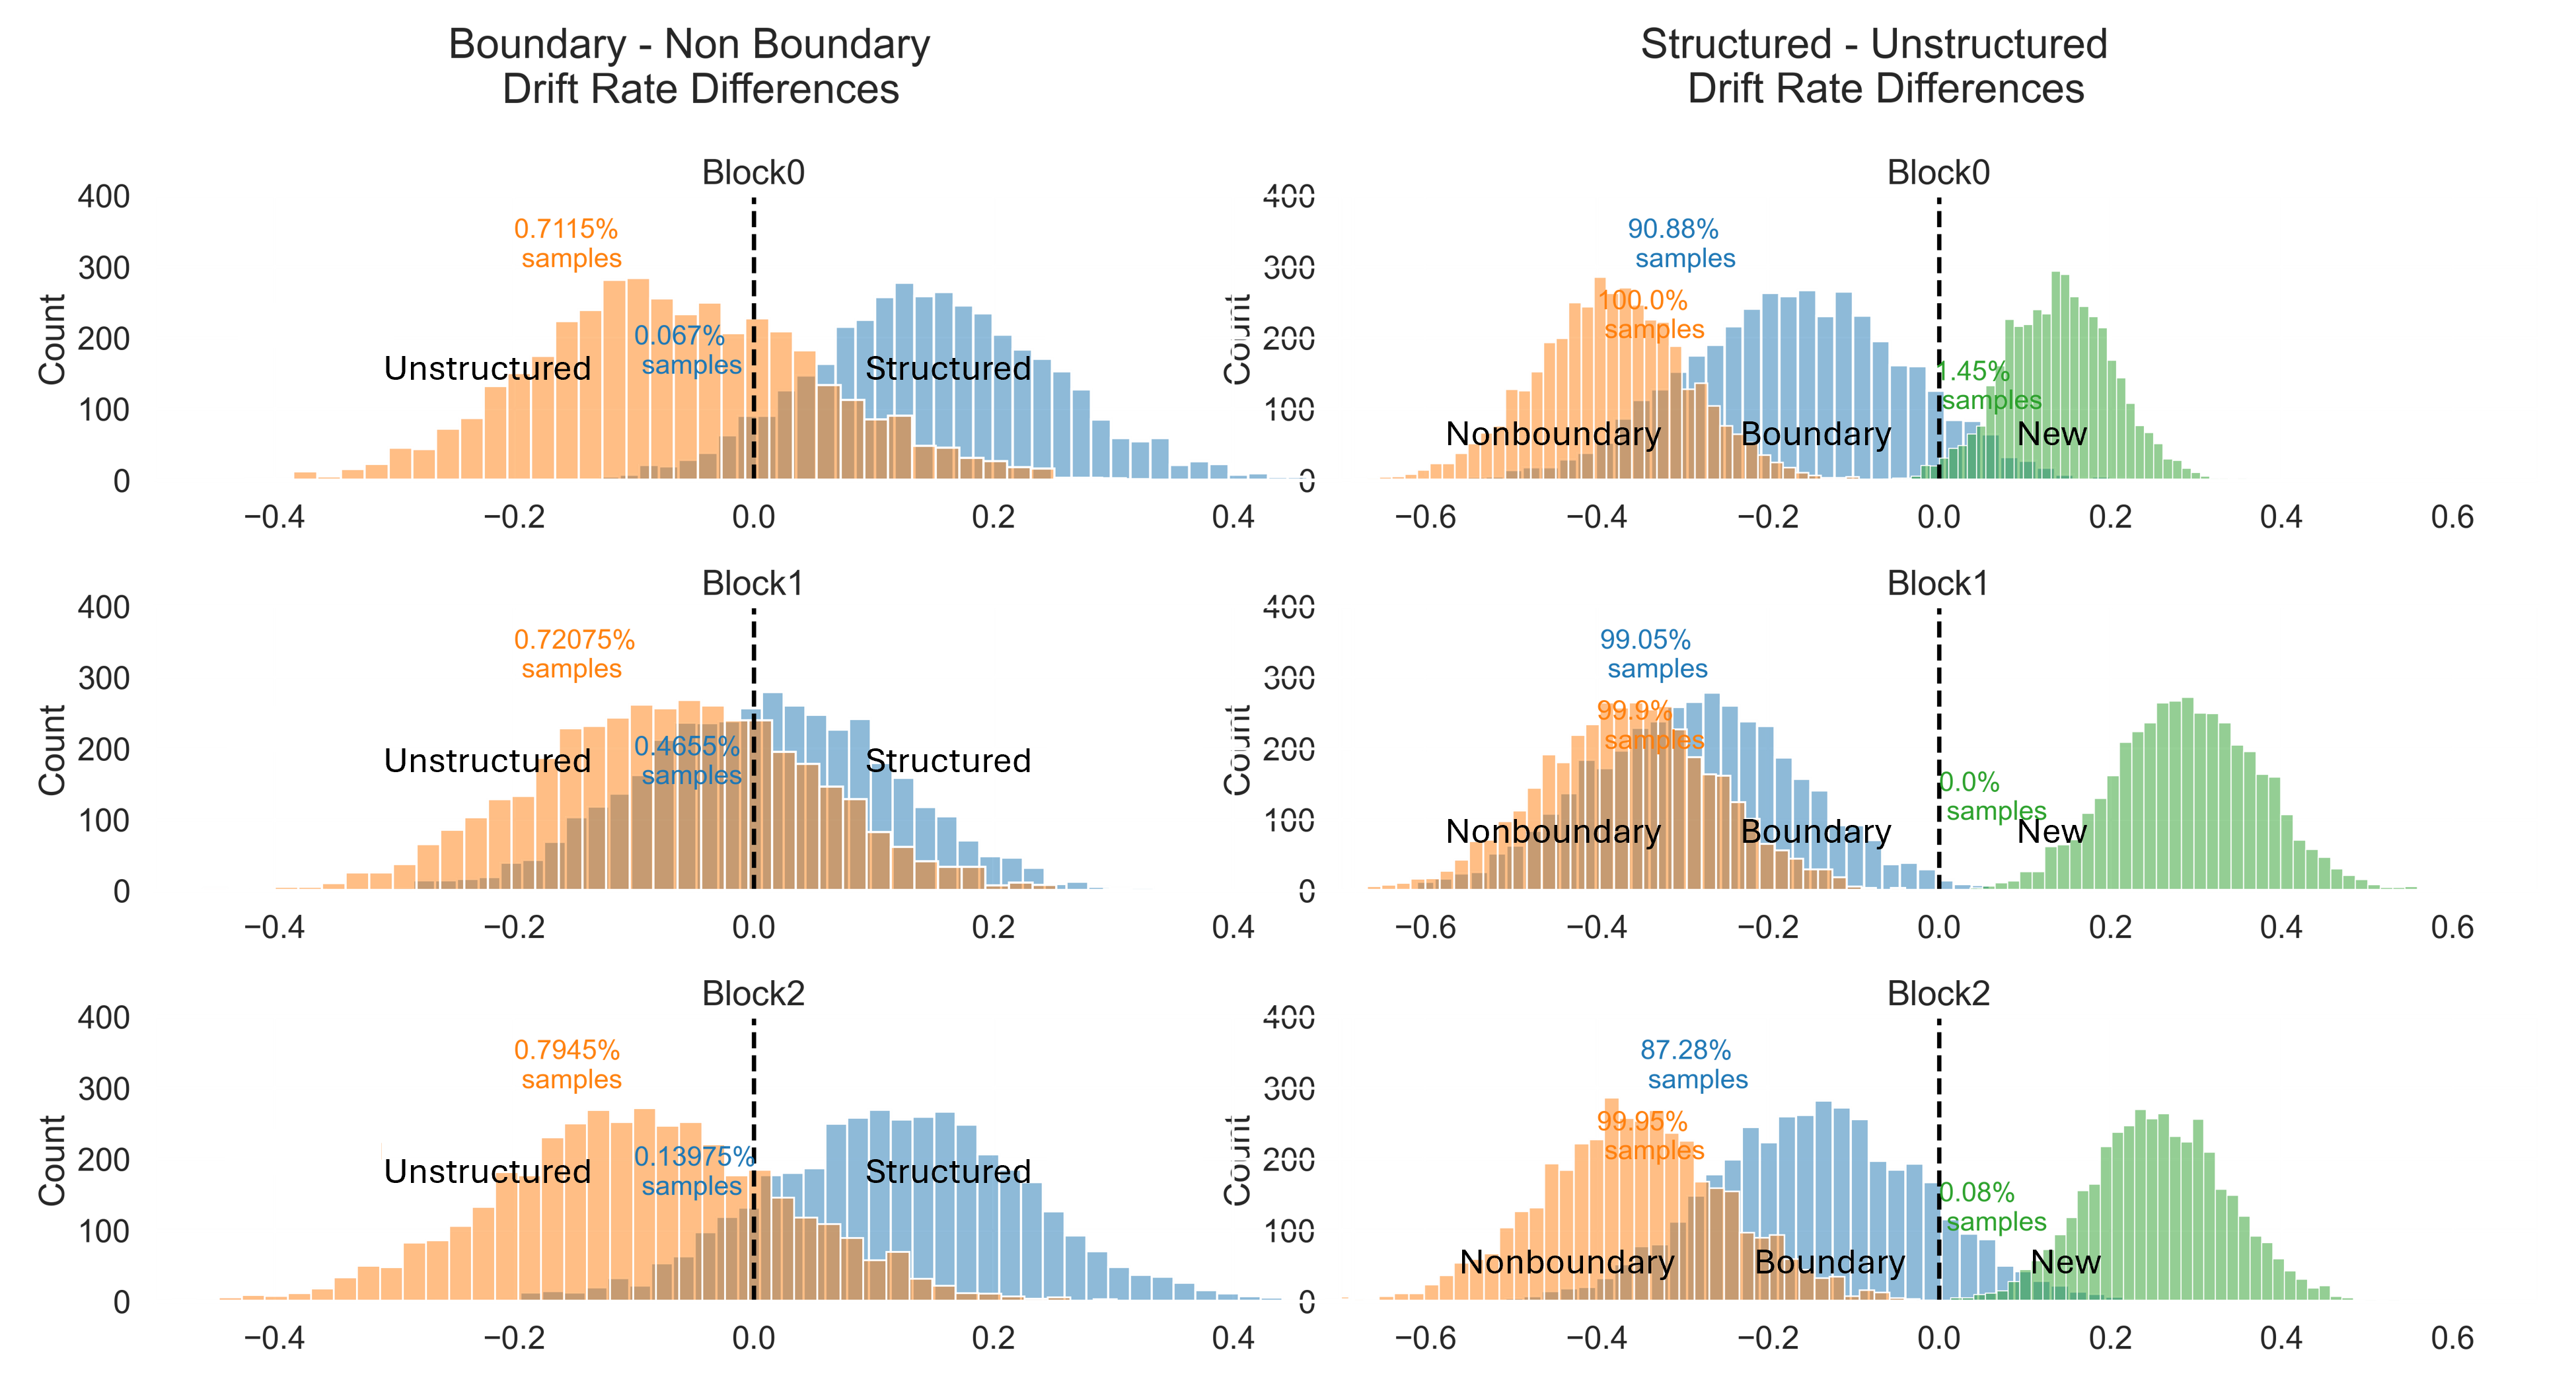
\includegraphics[width = \textwidth]{chapter_notebooks/chapter_3/figures/ddm_vdiff_comb.png}
    \caption{Drift rate differences. \textit{Left Panel.} Differences between boundary and non boundary nodes for structured and unstructured exposure conditions. \textit{Right Panel} Differences between drift rates between structured and unstructured conditions for each type of recognition memory stimulus. Figure text over each difference distribution depicts the proportion of posterior samples below 0.}
\end{figure}

Figure \ref{fig:ddm-drift-rates} shows the differences between drift rate parameters. The left panel shows that boundary nodes have a higher drift rate than non boundary nodes in the structured conditions relative to the unstructured conditions. The right panel shows the same effect within conditions. New items appear to have better drift rates than old items in the structured condition than the unstructured conditions. Finally, all drift rate differences are the lowest in the middle block indicating improved memory after 500 trials of exposure to the same stimuli relative to 250 trials after the first block. Increased differences in after the final block are likely owed to the Stroop distracter task prior to the final recognition test. 



\section{Modeling Boundary Distance Effects}
Another replicated finding in explicitly operationalized event boundary literature is an apparent increased separation of events across boundaries \cite{horner2016role,brunec2018boundaries,dubrow2013influence, ezzyat2011constitutes, heusser2018perceptual}. This separation of events across boundaries helps shape narratives in long term memory \cite{clewett2019transcending}.

It is unknown, however, whether the increased temporal separation across event boundaries generalizes to boundaries operationalized implicitly as well. Context models such as SR provide a mechanism to directly estimate perceived distance between events. Specifically, each cell in the SR matrix $M(s, s')$ indicates the future expected visit probabilities from state $s$ to state $s'$. Under the assumption that states closer to the current state are visited more often in a random walk than state farther, the probability $M(s, s')$ provides a direct estimate of perceived distance from node $s$ to $s'$. 

\begin{figure}[ht]
    \centering
    \label{fig:two_module_graph}
    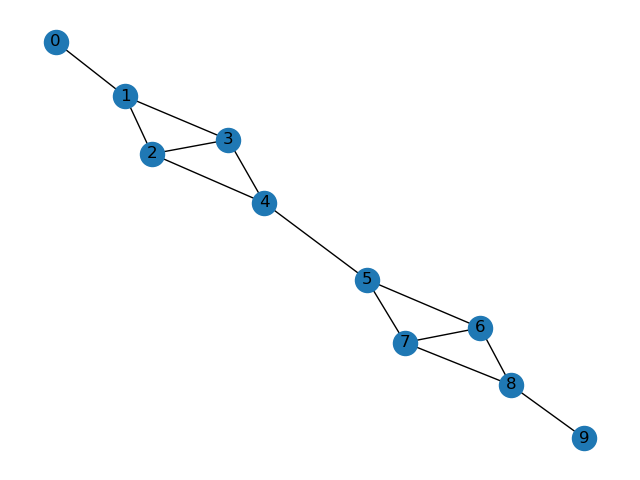
\includegraphics[width = \textwidth]{chapter_notebooks/chapter_3/figures/two_module_graph.png}
    \caption{Two module graph used for distance judgments.}
\end{figure}

To test whether cross boundary events are perceived to be farther from each other relative to within-boundary events graph in figure \ref{fig:two_module_graph} is used. The key transitions of interest that are compared in this graph are transitions at equal distances. Below I specify example transitions at 3 different distances however, for simulations and the experiment, all symmetrical transitions at those distances were tested. 
\begin{itemize}
    \item $0 \leftrightarrow 4$ vs $1 \leftrightarrow 5$ at shortest distance 3. 
    \item $1 \leftrightarrow 4$ vs $2 \leftrightarrow 5$ at shortest distance 2. 
    \item $2 \leftrightarrow 4$ vs $4 \leftrightarrow 4$ at shortest distance 1. 
\end{itemize}

\begin{figure}
    \centering
    \label{fig:SR-distance-estimate}
    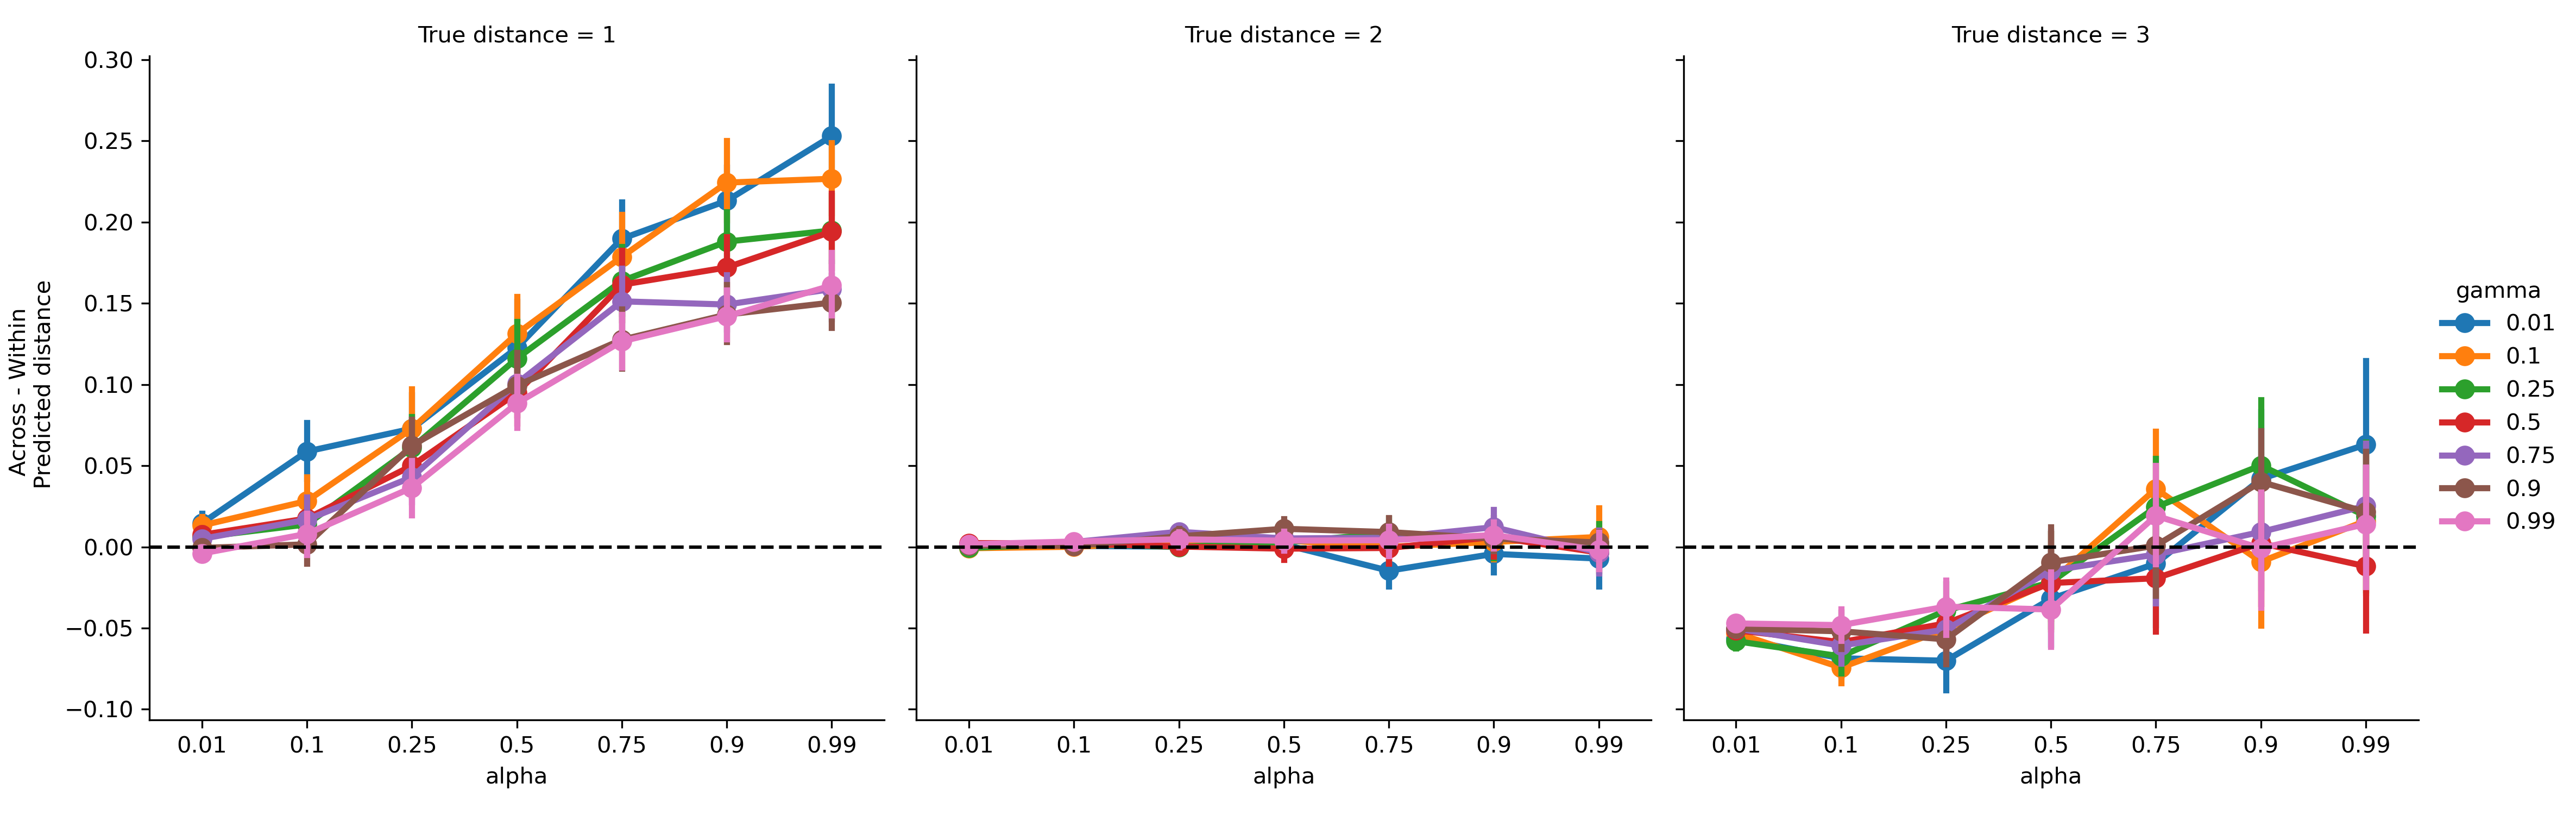
\includegraphics[width = \textwidth]{chapter_notebooks/chapter_3/figures/distance_predictions.png}
    \caption{SR predictions of distances across boundaries relative to distances within boundaries for nodes at true distance of 1, 2, and 3 and different parameter combinations.}
\end{figure}

SR estimate of distances is shown in figure \ref{fig:SR-distance-estimate}. Simulations predict that while boundary nodes themselves get perceptually farther with increased discount rate, neither of node-pairs at distance 2 or 3 that involve boundary nodes reliably show an increased cross-cluster distance.

\begin{figure}
    \centering
    \label{fig:SR-distance-estimate-entropy-boost}
    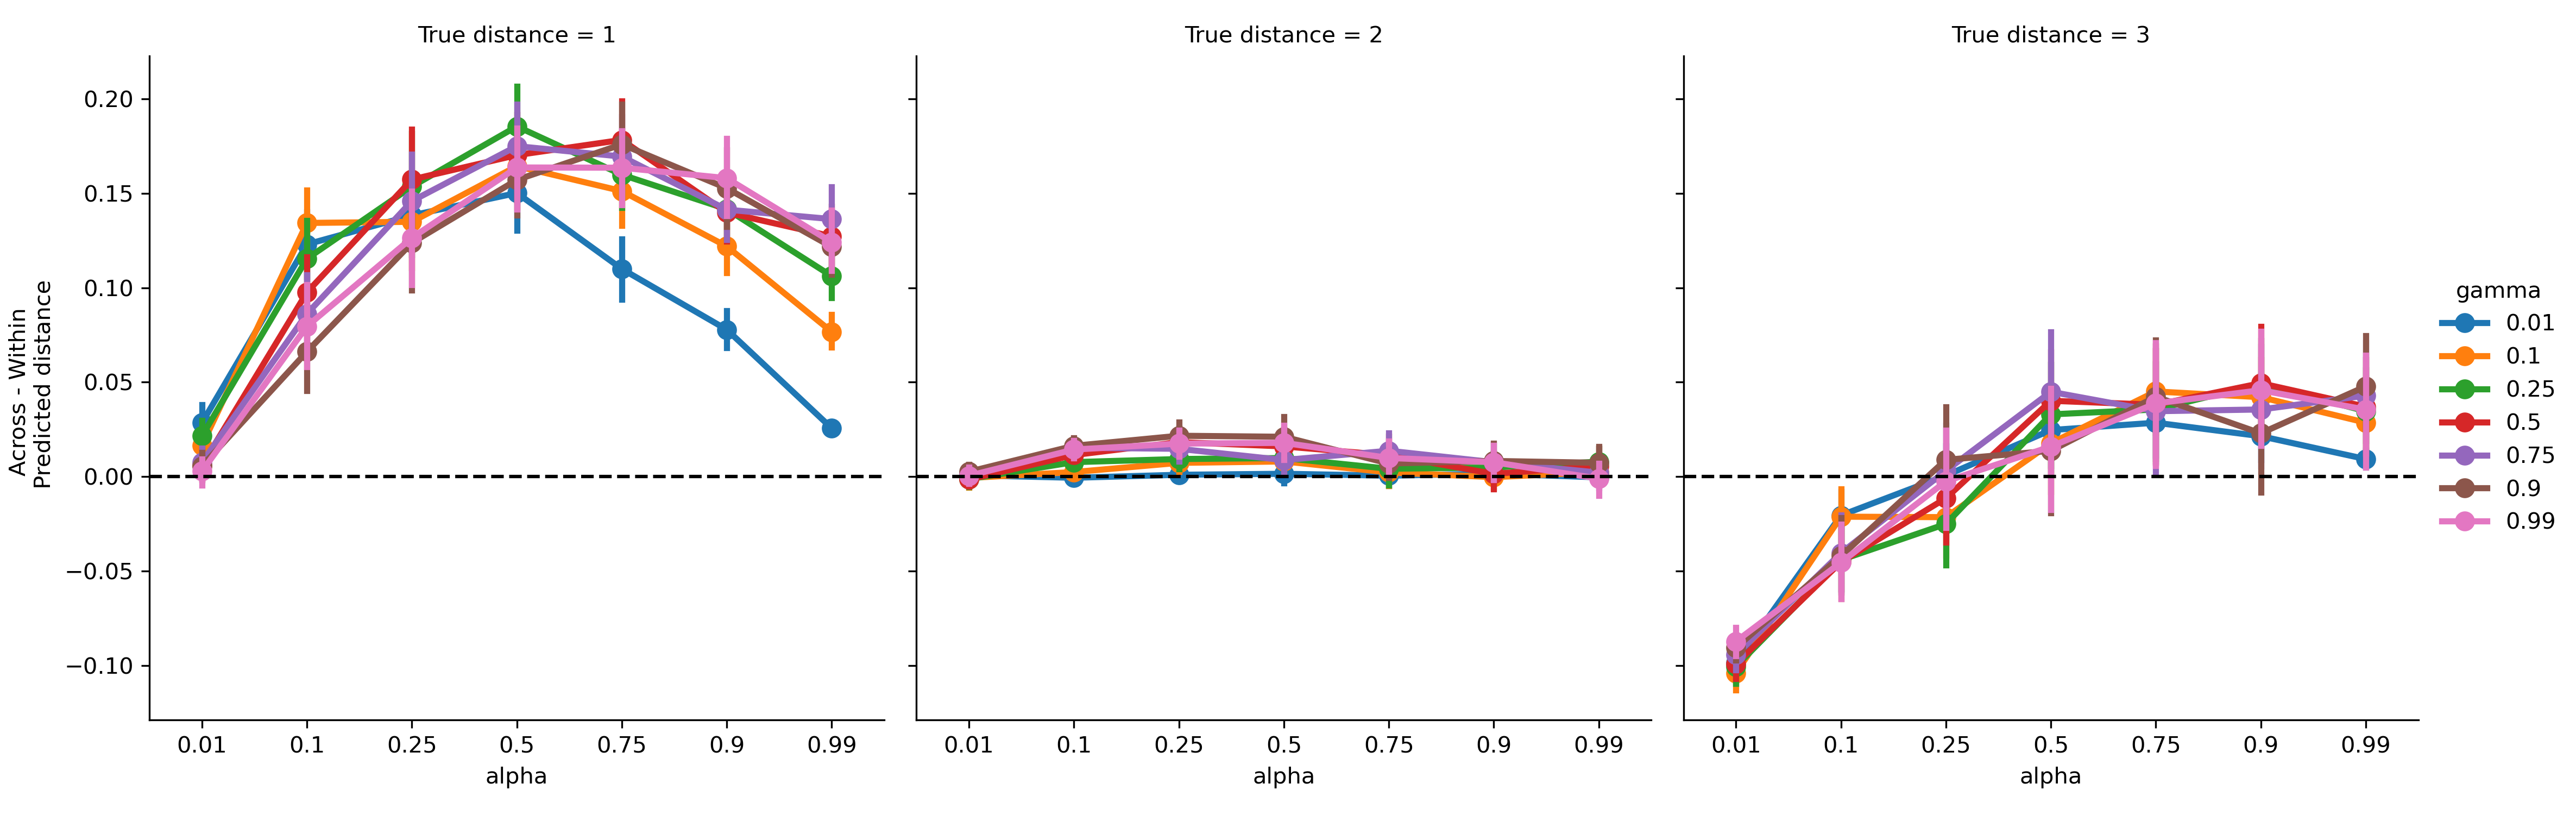
\includegraphics[width = \textwidth]{chapter_notebooks/chapter_3/figures/distance_predictions_entropyboost.png}
    \caption{SR predictions of distances across boundaries when boosted by node entropies relative to distances within boundaries for nodes at true distance of 1, 2, and 3 and different parameter combinations.}
\end{figure}

However, in a typical experience of the random walk, participants are shown to be slow at responding to boundary nodes; both due to higher entropy at boundary nodes (from chapter \ref{chapter-2-walk-lengths-modulate-statistical-learning}) and previously shown increased response times during transitions across temporal clusters \cite{lynn2020abstract,kahn2018network}. On average, a participant would typically spend more time at boundary nodes than non-boundary nodes thereby leading; thereby leading to increased perceived \textit{time} while crossing boundary nodes relative to staying within the cluster. Following the findings in chapter \ref{chapter-2-walk-lengths-modulate-statistical-learning}, this increased perceived time can be modeled through entropy difference between boundary and non-boundary nodes based on learned SR representations. This slowdown is simulated by multiplying average SR entropy of boundary nodes where they transitions cross boundaries and by multiplying the average SR entropy of non-boundary nodes where transitions stay within a cluster. predictions of differences in perceived distance are shown in figure \ref{fig:SR-distance-estimate-entropy-boost}.


Regardless of whether the distance measure is boosted by increased entropy at boundary nodes, it appears that boundary nodes themselves appear farther from each other relative to nodes within a cluster from that cluster's boundary node. Model predictions at other distances are mixed and dependent on parameters of the SR model. The next experiment tests whether the typical finding of increased perceived separation between cross cluster nodes (relative to within cluster nodes) is replicated in implicitly operationalized event boundary paradigms. A rigorous test of this formulation of the SR model is out of the scope of this dissertation. Furthermore, a lack of increased cross-cluster distance will provide no evidence for or against the current formulation of the SR model's role in representing distances between nodes. However, if such an increased cross-cluster distance is found, such an effect will serve as evidence \textit{against} the current formulation of the SR model's role in estimating temporal distances. 

\subsection{Methods}
\subsubsection*{Participants}
45 undergraduate students at the University of Massachusetts Amherst participated in this study. Participants were at least 18 years of age and were compensated via course credit. All study procedures were approved by the University Institutional Review Board. 

\subsubsection*{Design and Procedures}
Participants were randomly assigned to either a structured exposure or an unstructured exposure group. The overall experimental procedures were the same across both groups. 

Participants were first introduced to 10 randomly generated polygons and informed that these polygons are in their canonical orientation. Participants were asked to study these carefully and informed that they will make judgments about the orientation of these polygons in the coming phase. During the exposure phase, participants were shown one polygon at a time from the set of 10 they were introduced to. On each trial, the polygon was either rotated by 90 degrees or shown in its canonical orientation. Participants were asked to judge whether the polygon is rotated or not. 

The order of trials in exposure phase was determined based on a participant's group. 27 participants in the structured exposure condition were exposed to a stimulus stream generated by a random walk through the graph in figure \ref{fig:two_module_graph}. 18 participants in the unstructured exposure condition were shown a stimulus stream generated by randomly choosing any of the 10 polygons to be shown on any trial. The exposure phase lasted for 300 trials or 30 minutes, whichever came first. Participants were provided with an opportunity to take a self-paced break after 150 trials. 

During the test phase, participants were shown a triplet of polygons (see figure \ref{fig:exp3-design}). For each top polygon, participants were asked which of the bottom polygons was likely to appear first after seeing the polygon at the top in the stream they had experienced during exposure. The distance judgment phase lasted for 20 trials where 10 trials were consisted of the critical pairs (examples listed in the previous section) and 10 filler trials were based on randomly generated (non repeated) triplets. Responses to these filler trials were not analyzed.

\subsection{Results}

Figure \ref{fig:exp3-choice-results} provides an overview of the proportion of choices participants made to indicate a within cluster item is closer to the top item than a between cluster item. Descriptive statistics in table \ref{tab:exp3-choice-stats}

\begin{figure}
    \centering
    \label{fig:exp3-choice-results}
    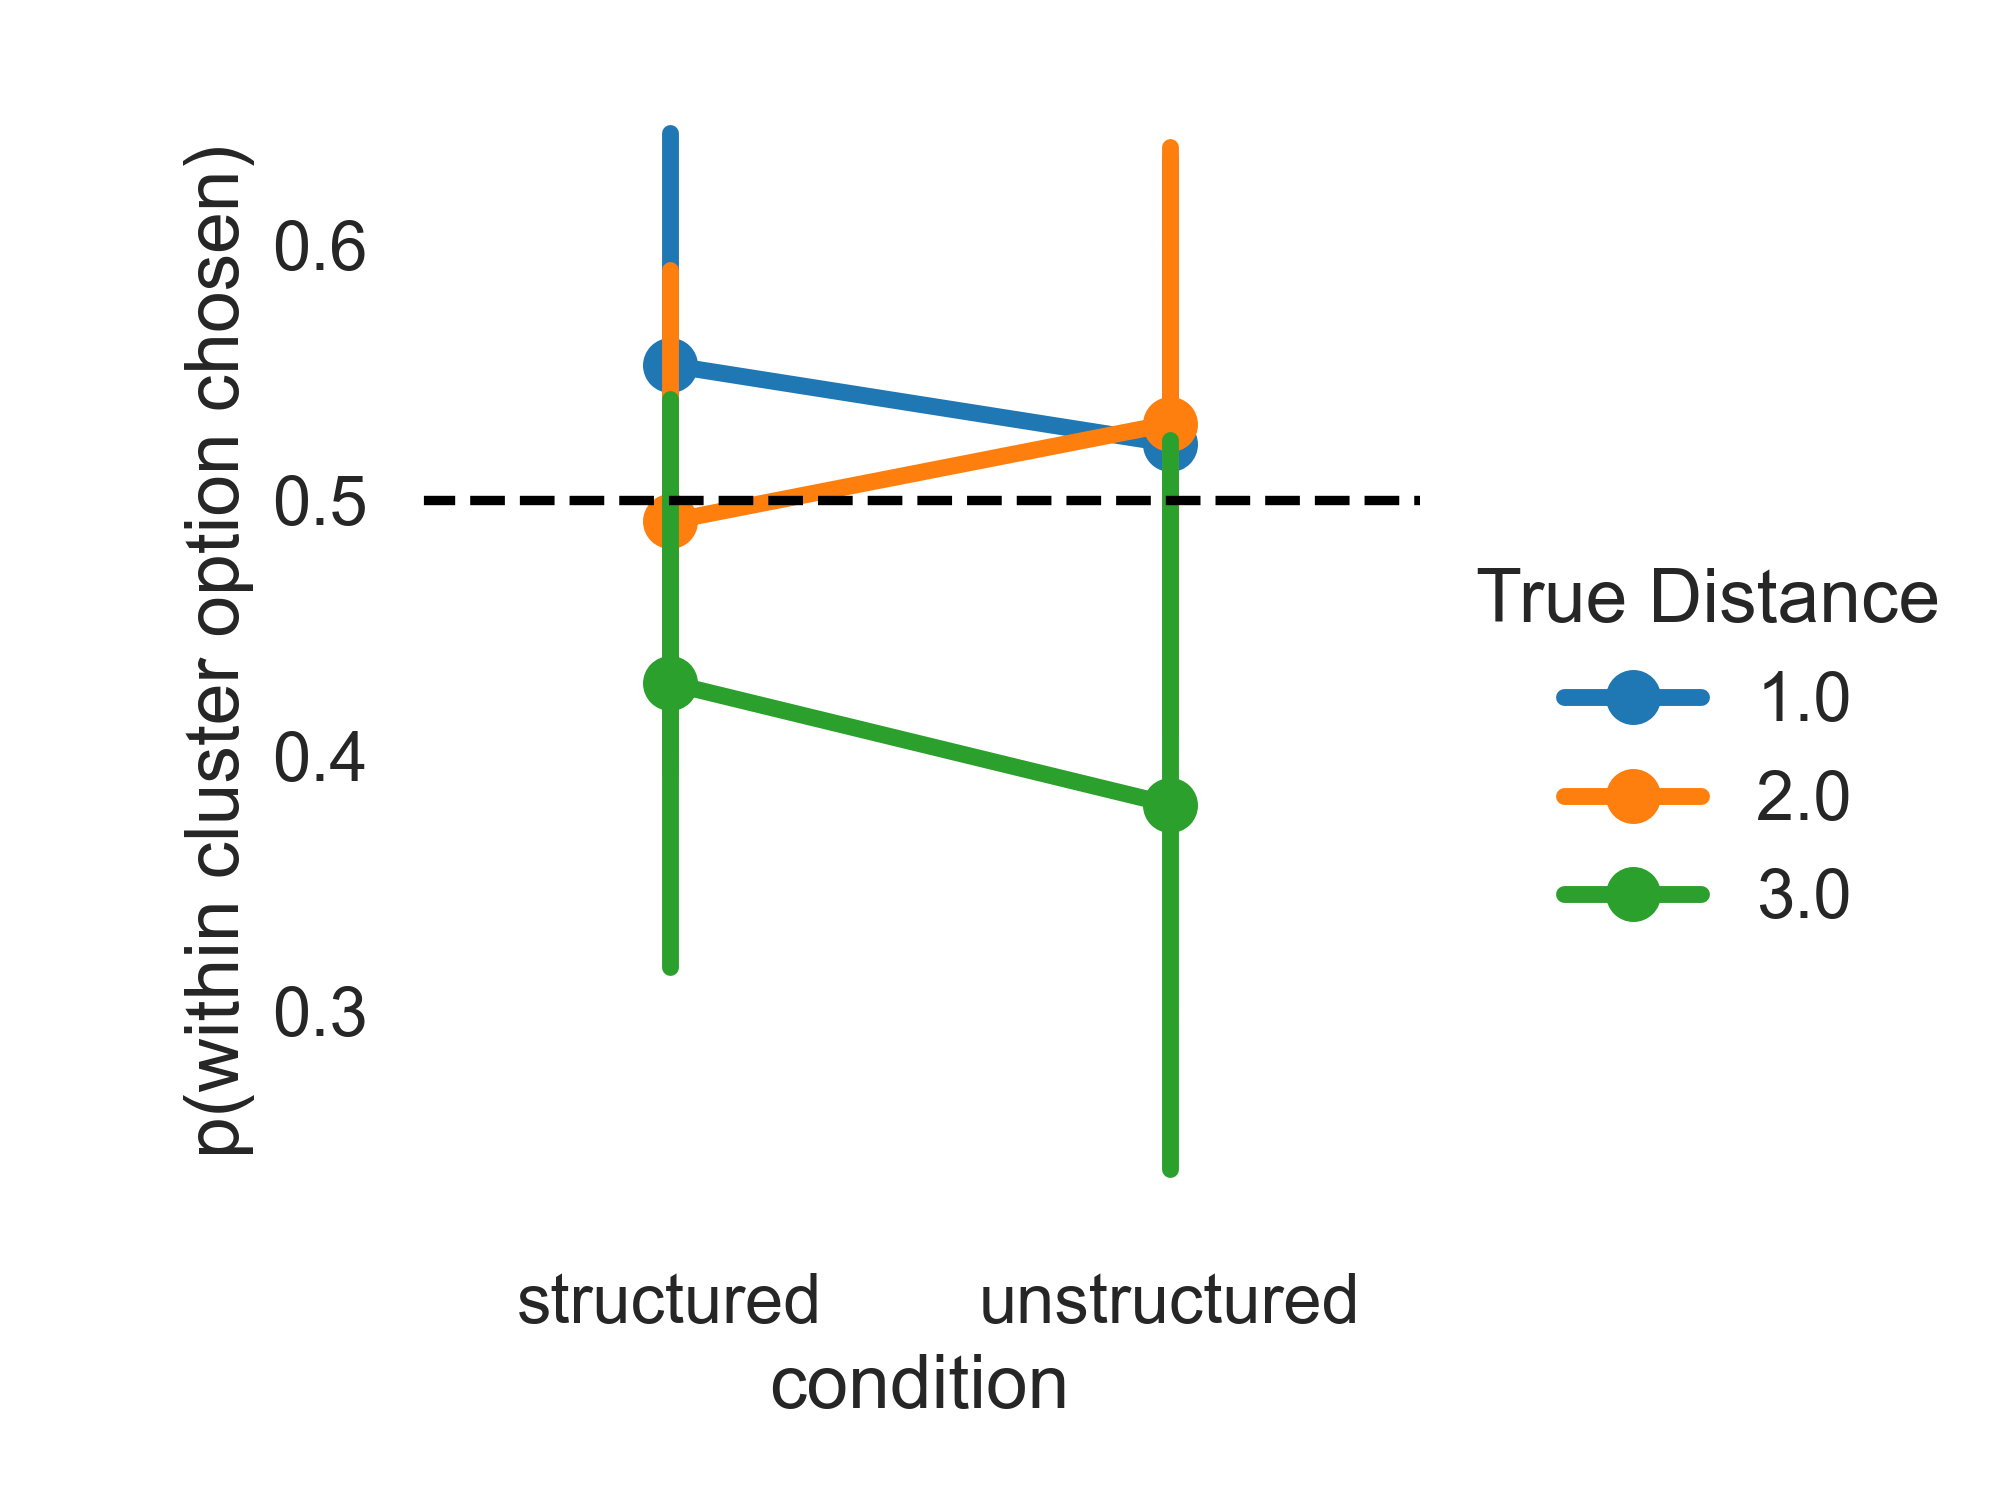
\includegraphics[width = \textwidth]{chapter_notebooks/chapter_3/figures/exp3_choice_results.png}
    \caption{Proportion of trials where the within cluster option was chosen when the distance between and within clusters were equal (ranging from a distance of 1, 2, and 3 connections).}
\end{figure}

\begin{table}
    \centering
    \label{tab:exp3-choice-stats}
    \begin{tabular}{llrr}
        \toprule
         &  & \multicolumn{2}{r}{within chosen} \\
         &  & mean & std \\
        condition & true distance &  &  \\
        \midrule
        \multirow[t]{3}{*}{structured} & 1.0 & 0.565 & 0.497 \\
         & 2.0 & 0.505 & 0.501 \\
         & 3.0 & 0.450 & 0.500 \\
        \cline{1-4}
        \multirow[t]{3}{*}{unstructured} & 1.0 & 0.528 & 0.501 \\
         & 2.0 & 0.533 & 0.501 \\
         & 3.0 & 0.521 & 0.503 \\
        \cline{1-4}
        \bottomrule
    \end{tabular}
     \caption{Proportions of trials where within cluster option at the same distance as the between cluster option was chosen.}   
\end{table}


\subsection{Discussion}

The primary goal of this chapter was to test whether findings in classical explicitly operationalized event boundary literature replicate when boundaries are operationalized implicitly, through temporal statistics. Shared properties between these two boundaries imply shared representations in memory thereby providing a framework for future research to study shared algorithmic processes that lead to formation of event boundaries. 

Under the representation of the SR to acquire boundaries in implicit learning tasks, two predictions were made: (1) Given the three-module graph structure (Figure \ref{fig:modular_graph}), items associated with boundary nodes will be remembered better than items associated with non-boundary nodes. And (2) Given the two-module graph structure (Figure \ref{fig:two_module_graph}), items within the same cluster should be picked at being closer than items across cluster only in a subset of circumstances. Specifically, the model predicts that items at within cluster items distance 1 are the most likely to be being closer and \textit{not} being farther. Furthermore, within cluster items at distance 2 should not be systematically be picked as being closer. Finally, 

The SR-based modeling approach provides a two advantages. First, qualitative pattern in data that matches model predictions provides support for the model and second, qualitative pattern in data that the model does \textit{predict} allows for disproving the model. Thus evidence in favor of the model should incorporate both support for better boundary item member in experiment 3a, and no unexpected distance judgment patterns (for a true distances of 2 and 3) in experiment 3b.

Results of experiments 3a and 3b thus provide support for an SR representation of implicit event boundaries. Furthermore, better memory for boundary items provides evidence in favor of similar representations of implicit boundary events compared to explicit boundary events. On the other hand, however, distance judgment results in this implicit event boundary task do not directly compare with findings from explicit boundary literature. It is possible that lack of an ongoing verbalizable narrative in randomly generated polygons impacts how well neighboring items are bound with each other thereby not allowing us to detect an effect.

DDM is one (highly successful) model of memory that incorporates response time. Other models incorporating response in choice reaction tasks. Several other sequential sampling models can be used in this formulation to provide evidence of better memory strength for boundary items. Most notably, a direct extension of the GCM model for recognition memory is the Exemplar Based Random Walk (EBRW) model \cite{nosofsky2011short}. 